\documentclass[11pt,a4paper]{article}
\usepackage[margin=25mm]{geometry}
\usepackage{amsmath,amssymb,amsthm,mathtools,bm}
\usepackage[T1]{fontenc}
\usepackage{lmodern,microtype,booktabs,enumitem,graphicx,array,longtable}
\usepackage{xcolor,xurl}
\usepackage[colorlinks=true,linkcolor=blue!50!black,urlcolor=blue!50!black,citecolor=blue!50!black]{hyperref}
\hypersetup{pdftitle={The one-sided CHSH measure under local filtering: exact supremum, violation criterion and a least-eigenvalue formula},pdfauthor={Dev D. Goyal},pdfsubject={Exact solution of the one-sided hidden CHSH measures of Ducuara, Susa and Skrzypczyk, with Lean proofs for actual two-qubit density matrices}}
\newtheorem{theorem}{Theorem}
\newtheorem{lemma}[theorem]{Lemma}
\newtheorem{corollary}[theorem]{Corollary}
\newtheorem{proposition}[theorem]{Proposition}
\theoremstyle{remark}\newtheorem{remark}[theorem]{Remark}
\DeclareMathOperator{\tr}{tr}\DeclareMathOperator{\spec}{spec}
\DeclareMathOperator{\rank}{rank}\DeclareMathOperator{\ran}{ran}
\DeclareMathOperator{\diag}{diag}\DeclareMathOperator{\adj}{adj}
\newcommand{\R}{\mathbb R}\newcommand{\C}{\mathbb C}
\newcommand{\HH}{\mathcal H}\newcommand{\BB}{\mathcal B}\newcommand{\JJ}{\mathcal J}
\newcommand{\norm}[1]{\left\lVert#1\right\rVert}
\newcommand{\ip}[2]{\langle #1,#2\rangle}
\title{The one-sided CHSH measure under local filtering:\\
exact supremum, violation criterion and\\ a least-eigenvalue formula}
\author{Dev D. Goyal}
\date{3 November 2026}
\begin{document}
\maketitle
\begin{abstract}
Ducuara, Susa and Skrzypczyk (Phys.\ Rev.\ A \textbf{110}, 022435, 2024)
defined the one-sided hidden CHSH measures $HB_A$ and $HB_B$ of a
two-qubit state, the largest normalized CHSH value obtainable when only one
party applies an invertible local filter (their Eq.~(9)), and noted that no
closed formula was known. We solve this optimization for every two-qubit
state. After whitening the filtering party's marginal, the supremum equals
the maximum of one explicit quadratic function over a compact set of pairs
of vectors in $\R^3$; it is attained by an invertible filter whenever it
exceeds the local bound, and in general may be only a supremum. Writing the
whitened data as an other-party Bloch vector $c$ and correlation matrix
$D$, put $A=DD^{\mathsf T}$, $K=A-\norm c^2 I$, $C=[Dc]_\times$ and
$\alpha=\tr A-\norm c^2$. One-sided violation is possible only if
$\alpha>1$, and throughout that region the squared supremum is
$\tr A-\lambda_{\min}(A+CK^{-1}C)$, the least eigenvalue of an explicit
symmetric $3\times3$ matrix, with an explicit optimal filter. Hence
violation occurs exactly when $\alpha>1$ and $A+CK^{-1}C-(\tr A-1)I$ is
not positive semidefinite, a test by three polynomial signs. For
$\alpha\le1$ the value is at most one and is the largest of at most four
algebraic candidates: values at the admissible roots of a cubic pencil and a
boundary radius determined by a specified root of a secular equation of degree
at most six. We add a
rational formula for states of rank at most two, the exact one-sided value
$\max\{1,2p/(2-p)\}$ for the quasi-distillable family of the 2024 paper,
and exact success-probability trade-offs. Lean~4 with Mathlib proves, for
every positive semidefinite trace-one complex $4\times4$ matrix, arbitrary
invertible complex filters on either party and arbitrary traceless
Hermitian involutive qubit observables, the supremum, the violation
criterion, the least-eigenvalue formula and invertible attainment; the
secular-root boundary algorithm and the further results have conventional
proofs and independent checks.
\end{abstract}

\setcounter{tocdepth}{1}
\tableofcontents

\section{Introduction}
\label{sec:intro}

\subsection{The question in plain terms}

Two parties, Alice and Bob, share a two-qubit state $\rho$ and run a CHSH
Bell test. A state that does not violate the CHSH inequality may still do
so after \emph{local filtering}: each party applies a two-outcome
measurement, and the parties keep the runs in which a designated outcome
occurred. Filtering by both parties is completely understood: the
optimal filters bring the state to a Bell-diagonal normal form, and the
resulting ``hidden'' CHSH value has a closed formula~\cite{verstraetewolf,
klm,ducuara}. Ducuara, Susa and Skrzypczyk~\cite{ducuara} asked what
happens when only \emph{one} party may filter, a situation natural in
semi-device-independent settings. They defined
\begin{equation}
 HB_W(\rho)=\max_{f_W}B(\rho'_{F_W}),\qquad W\in\{A,B\},
 \label{eq:dss9}
\end{equation}
their Eq.~(9), where $B$ is the CHSH value normalized to local bound $1$
and Tsirelson bound $\sqrt2$, $f_W\in\mathrm{GL}(2,\C)$ acts on the party
$W$ only, and $\rho'_{F_W}$ is the normalized filtered state. They
observed that ``unlike the standard hidden correlations, \dots\ there are
currently no closed formulas for the one-sided versions'', and listed
closed formulas for these measures among their open questions. Below we
write $B_A^*$ for $HB_A$.

\subsection{The answer in plain terms}

The filtering party's marginal can first be made maximally mixed
(``whitened'') without changing the set of reachable states. After that,
a filter is described by a vector $u$ in the Bloch ball, and the optimal
CHSH value of the filtered state is a ratio of quadratic expressions. A
change of variables (Section~\ref{sec:compact}) turns the whole problem,
including the choice of the two measured directions, into the maximum of a
single quadratic function $f(n,v)$ over pairs of vectors with $\norm n=1$,
$n\perp v$ and $\norm v\le1$. Points with $\norm v=1$ correspond to
rank-one limits of invertible filters, which is why the ``maximum'' in
Eq.~\eqref{eq:dss9} is in general only a supremum.

Physical positivity then does most of the work. A spin-flip Gram identity
shows that a one-sided violation needs the purity quantity $\alpha$ of
the whitened state to exceed one, and that for $\alpha>1$ the maximum of
$f$ is interior and is given by completing a square: the answer is one
explicit $3\times3$ least eigenvalue. For $\alpha\le1$ no violation is
possible; the exact sub-classical value is still determined, as the largest
of finitely many algebraic candidates.

\subsection{Main results}
\label{sec:main-results}

Let $\rho$ have Bloch data $(a,b,T)$ and mixed Alice marginal
($\norm a<1$). Whitening Alice gives canonical data $(c,D)$
(Equation~\eqref{eq:canonicalbloch}); put
\[
 A=DD^{\mathsf T},\quad s=\norm c^2,\quad C=[Dc]_\times,\quad K=A-sI,\quad
 \alpha=\tr A-s,\quad M=A+CK^{-1}C.
\]
In original coordinates $\alpha=(\norm T_F^2-\norm b^2)/(1-\norm a^2)$
(Equation~\eqref{eq:ext-raw-alpha}). Bob's measure is obtained by exchanging
the parties, that is, exchanging $a$ and $b$ and transposing $T$.

\begin{enumerate}[label=\textbf{\Alph*.},leftmargin=2em]
\item \textbf{Exact supremum for every state.} $(B_A^*)^2$ equals the
maximum of the explicit quadratic $f$ of Equation~\eqref{eq:f} over the
compact domain~\eqref{eq:domain}; if Alice's marginal is pure, the state
is a product and $B_A^*=\norm b$, attained
(Equations~\eqref{eq:compactreduction} and~\eqref{eq:puremarginal}).
\emph{Lean-checked.}
\item \textbf{Least-eigenvalue formula where violation is possible.}
If $\alpha>1$ then $K\succ0$ and
\[
 (B_A^*)^2=\tr A-\lambda_{\min}(M),
\]
attained by the invertible filter of Equation~\eqref{eq:ext-shortcut-filter}
(Theorem~\ref{thm:ext-shortcut}). \emph{Lean-checked.} The same holds when
$K+iC\succ0$ (conventional).
\item \textbf{Exact violation criterion.} $B_A^*>1$ if and only if
$\alpha>1$ and $M-(\tr A-1)I\not\succeq0$; a violating supremum is always
attained by an invertible filter. Hidden one-sided activation additionally
requires $s_1(T)^2+s_2(T)^2\le1$ for the original state. \emph{Lean-checked.}
The equivalent test by the signs of three polynomials in the Bloch data,
including a version in rational steering-ellipsoid data
(Theorem~\ref{thm:ext-polynomial}), is conventional.
\item \textbf{All remaining states.} For $\alpha\le1$, $(B_A^*)^2\le1$, and
for every state $(B_A^*)^2$ is the largest of the boundary radius
$E=\max_{\norm u=1}\norm{c+D^{\mathsf T}u}^2$ and at most three values
$\tr A-\lambda$ at admissible roots $\lambda$ of a cubic pencil
(Theorem~\ref{thm:main}). The finite-candidate statement is
\emph{Lean-checked}, with $E$ represented as an attained maximum over the
sphere; the explicit evaluation of $E$ by a secular equation and the
admissibility tests are conventional.
\item \textbf{Further exact results} (conventional, with exact and numerical
checks): for $\rank\rho\le2$,
$(B_A^*)^2=1+\max(0,\norm T_F^2+\norm a^2-\norm b^2-1)/(2(1-\norm a^2))$
(Theorem~\ref{cor:ext-low-rank}); $B_A^*=\sqrt2$ exactly for pure entangled
states; a three-regime classification at $B_A^*=1$
(Theorem~\ref{thm:ext-threshold}); the exact one-sided value
$(B_A^*)^2=(B_B^*)^2=\max\{1,2p/(2-p)\}$ for the quasi-distillable family
$p\,\psi^-+(1-p)|00\rangle\langle00|$ of~\cite{ducuara}; exact
success-probability trade-offs for canonical and original inputs
(Sections~\ref{sec:ext-probability} and~\ref{sec:r3-success}); and
convexity, noise-scaling and stability properties
(Section~\ref{sec:ext-stability}).
\end{enumerate}

\paragraph{What is closed-form and what is algorithmic.}
Results B and C are closed formulas: a least eigenvalue of an explicit
symmetric $3\times3$ matrix (a root of an explicit cubic,
Corollary~\ref{cor:ext-rational-cubic}) and three polynomial sign
conditions. They cover every state for which one-sided violation is
possible, and every state with $\alpha>1$ whether or not it violates. The
rank-two formula and the pure-marginal value are also closed. For
$\alpha\le1$ the value never exceeds one, and its exact value is
algorithmic but finite: compute the cubic pencil roots, test their
admissibility by small singular-value problems, evaluate $E$ through the
unique root above the top eigenvalue of $A$ of a secular equation of degree
at most six (or the explicit hard-case expression), and take the largest.
In the Lean development the value for $\alpha\le1$ appears as this finite
candidate set with $E$ an attained maximum over a sphere; the secular-root
construction of $E$ is not formalized.

\paragraph{Formal scope.}
The Lean statements quantify over every positive semidefinite trace-one
$4\times4$ complex matrix, every complex $2\times2$ filter with nonzero
determinant on either party, normalized by the actual trace, and every
quadruple of traceless Hermitian involutive qubit matrices as measurement
observables; Appendix~\ref{sec:verification} lists the declarations and
what remains conventional.

\paragraph{Reading guide.}
Section~\ref{sec:prior} records prior work and priority.
Section~\ref{sec:setting} fixes notation and reduces to a whitened marginal;
Section~\ref{sec:compact} proves the compact reduction (Result~A).
Sections~\ref{sec:ext-gram}--\ref{sec:ext-shortcut} prove Result~B, which is
all that is needed for the violation question. Section~\ref{sec:formula}
treats every state (Result~D); the proof of its finite-candidate theorem is
in Appendix~\ref{sec:proof-general}. Section~\ref{sec:attainment} gives optimal filters, attainment
and the violation criteria (Result~C), and the later sections contain the
further results. Appendix~\ref{sec:verification} describes the
verification.

\section{Prior work and priority}
\label{sec:prior}

\paragraph{The question.} The measures~\eqref{eq:dss9} and the normalization
of $B$ are those of Ducuara, Susa and Skrzypczyk~\cite{ducuara}. The
optimal CHSH value over projective qubit measurements is the Horodecki
formula $B(\rho)^2=s_1(T)^2+s_2(T)^2$~\cite{horodecki1995}, used
throughout. The Lorentz representation of local filtering is due to
Verstraete, Dehaene and De~Moor~\cite{verstraete}; the optimal bilateral
filters and the Bell-diagonal normal form are due to Kent, Linden and
Massar~\cite{klm} and Verstraete and Wolf~\cite{verstraetewolf}.
Bilateral hidden-nonlocality criteria include those of Pal and
Ghosh~\cite{palghosh} and Li et al.~\cite{li2017}; they optimize both
filters and do not solve~\eqref{eq:dss9}. Whitening one party identifies
its filtering orbit with pure inputs to the qubit channel whose Choi state
is the whitened state, so one-sided activation is equivalent to failure of
the CHSH-breaking property for that channel; Zhang, Araiza Bravo, Lorenz
and Chitambar~\cite{zhang} solve the unital case (recovered here at
$c=0$) and several nonunital families, including the amplitude-damping
threshold, and state that no general analytical criterion was known for
nonunital channels. Kumari et al.~\cite{kumari} relate CHSH breaking to
incompatibility breaking.

\paragraph{Ingredients that are not new.}
The bound of the CHSH value by a conditional purity (negative conditional
R\'enyi-2 entropy is necessary for violation) is due to
R.~Horodecki, P.~Horodecki and M.~Horodecki~\cite{horodecki1996}. The
rank-two formula uses the Ruskai--Szarek--Werner normal form of qubit
channels~\cite{ruskai2002}. The boundary radius is a trust-region
subproblem, evaluated by the classical secular equation and hard case of
Mor\'e and Sorensen~\cite{more}. The certificate hierarchy in
Section~\ref{sec:r3-success} uses the matrix Positivstellensatz of Hol and
Scherer~\cite{holscherer2005}.

\paragraph{Omega Institute record on Milne's Conjecture~1 (note dated 3 November 2026).}
The Omega Institute's public repository
\texttt{the-omega-institute/trureturing} records a claimed Lean proof of
Conjecture~1 of Milne, Jennings, Jevtic and Rudolph~\cite{milne}, the
bound of the CHSH value by the length $c$ of the centre of the steering
ellipsoid~\cite{jevtic} for every two-qubit state; the dossier for its issue \#16558 was committed on
14 October 2026 at 08:40:22 UTC~\cite{dossier}. That record touches this
paper in two places. First, its proof uses a plane-purity identity and the
covariance of a conditional purity under one-sided filtering; with the
parties exchanged these are Equations~\eqref{eq:ext-plane-purity}
and~\eqref{eq:ext-delta-covariance} of Proposition~\ref{prop:ext-purity},
which we therefore do not claim as new. Second, Result~1
of~\cite{ducuara} deduces the impossibility of one-sided violation for
centre lengths above $1/2$ from Conjecture~1, so the claimed proof makes
that criterion unconditional; for the quasi-distillable family it already
gives the inaccessibility interval $0<p\le2/3$ (Section~\ref{sec:ext-axial}),
for which no priority is claimed. The package
\href{https://github.com/dvgyl/math-and-theory/tree/main/papers/physics/chsh-steering-ellipsoid}{chsh-steering-ellipsoid}
of this collection treats Conjecture~1 as well. Neither record, as read on
3 November 2026, contains the one-sided supremum, the exact violation
criterion, the least-eigenvalue formula or the finite candidate formula,
and Conjecture~1 is not used here. The Omega dossier lists bounds on the
CHSH value by the full steering ellipsoid, rather than its centre alone, as
open. We have not checked
the Omega Institute's Lean proof and describe it as claimed.

\paragraph{What is new here, as far as we found.} The compact reduction,
the finite spectral formula for every state, the least-eigenvalue formula
with automatic feasibility in the region $\alpha>1$, the exact one-sided
violation criterion and its polynomial form, the rank-two formula for the
one-sided measure, the exact one-sided values for the quasi-distillable
family, the success-probability trade-offs and the Lean development. A
bounded literature search did not find these results; this does not
establish priority, and a specialist review remains appropriate.

\section{Setting, notation and the canonical reduction}
\label{sec:setting}

Write a two-qubit density matrix as
\begin{equation}
 \rho=\frac14\sum_{\mu,\nu=0}^3 R_{\mu\nu}\sigma_\mu\otimes\sigma_\nu,
 \qquad R=\begin{pmatrix}1&b^T\\a&T\end{pmatrix}.
\end{equation}
We use precisely the normalization of Equations (2) and (9) of Ducuara--Susa--Skrzypczyk~\cite{ducuara}; the expression of the optimal CHSH value through the two largest singular values $s_1(T)\ge s_2(T)$ of the correlation matrix is the Horodecki criterion~\cite{horodecki1995}:
\begin{equation}
 B(\rho)=\sqrt{s_1(T)^2+s_2(T)^2},\qquad
 B_A^*(\rho)=\sup_{F\in\mathrm{GL}(2,\C)}
 B\!\left(\frac{(F\otimes I)\rho(F^\dagger\otimes I)}
 {\tr[(F^\dagger F\otimes I)\rho]}\right).
 \label{eq:definition}
\end{equation}
The CHSH local bound is $1$, the Tsirelson bound is $\sqrt2$, and the usual unnormalized Bell expression is $2B$. Only the traceless spin observables in the paper's definition are being optimized. Consequently $B_A^*$ can be less than $1$, or even zero. It is incorrect to insert a universal floor of $1$.

The paper writes a maximum over invertible filters. A supremum is necessary: the maximizing sequence can converge to a rank-one filter. All positive scalar multiples of a filter yield the same normalized state; a scalar can always make $F^\dagger F\le I$.

If $\rho_A=(I+a\cdot\sigma)/2$ is invertible, set
\begin{equation}
 W=(2\rho_A)^{-1/2},\qquad
 \rho_c=(W\otimes I)\rho(W\otimes I),\qquad
 R_c=\begin{pmatrix}1&c^T\\0&D\end{pmatrix}.
 \label{eq:canonical}
\end{equation}
The trace of $\rho_c$ is $1$. Since $W$ is invertible, composing filters with $W$ gives a bijection of the unilateral filtering orbit. Thus it suffices to compute $B_A^*(\rho_c)$. For direct Bloch-data evaluation, with $r_a=\sqrt{1-\norm a^2}>0$,
\begin{align}
 c&=\frac{b-T^Ta}{r_a^2},\\
 D&=\frac{\left(r_a I+\dfrac{aa^T}{1+r_a}\right)T-ab^T}{r_a^2}.
 \label{eq:canonicalbloch}
\end{align}
No inverse of $T$, $D$, or the full density matrix is required.

If $\rho_A$ is pure, positivity implies $\rho=\rho_A\otimes\rho_B$. Every nonzero invertible Alice filter leaves a pure Alice marginal and the same Bob marginal. Hence
\begin{equation}
 \boxed{B_A^*(\rho)=\norm b\quad\text{when }\norm a=1,}
 \label{eq:puremarginal}
\end{equation}
and the value is attained. For Bob-only filtering, interchange $a,b$ and transpose $T$ throughout.

\paragraph{Canonical data.}
From the canonical data $(D,c)$ define
\begin{equation}
 A=DD^T,\quad s=c^Tc,\quad d=Dc,\quad C=[d]_\times,\quad K=A-sI,
 \qquad [d]_\times x=d\times x.
 \label{eq:data}
\end{equation}
Thus $A,K$ are real symmetric, while $C^T=-C$. Throughout we also use the \emph{boundary radius}, the largest squared length of a Bloch vector to which a rank-one Alice effect steers Bob:
\begin{equation}
 E=\max_{\norm u=1}\norm{c+D^Tu}^2;
 \label{eq:boundarydescription}
\end{equation}
Section~\ref{sec:boundary} evaluates it in closed form up to one scalar root.

\section{The compact reduction}
\label{sec:compact}

\paragraph{Idea.} A filter on Alice acts on the Pauli coordinates by a Lorentz transformation followed by normalization, and the CHSH value of the output is the sum of the two largest squared singular values of its correlation matrix. Fixing the two measured directions and choosing the remaining filter freedom optimally turns the supremum over all invertible filters into the maximum of one explicit quadratic function $f(n,v)$ over a compact set of pairs of vectors in $\R^3$. Everything else in the paper is an analysis of this maximum.

\subsection{Filtering and a Lorentz two-plane}

The usual Lorentz representation of local filtering follows from the Pauli determinant identity~\cite{verstraete}: for a Hermitian matrix $X=x_0I+x\cdot\sigma$,
$\det X=x_0^2-\norm x^2$. Conjugation by an invertible filter, divided by $|\det F|$, preserves this quadratic form and the future cone. Thus Alice filtering acts on the real matrix $R$ by a Lorentz matrix, followed by trace normalization.

For a canonical marginal the denominator is the time coordinate $w_0$ of the timelike row. Choose the first two spatial rows to be the two maximizing directions in the Ky Fan formula for $B^2$; write them as $(x_0,X)$ and $(y_0,Y)$. Let the omitted spatial row have time coordinate $z_0$. Lorentz orthogonality gives
\begin{equation}
 X^TX=1+x_0^2,\quad Y^TY=1+y_0^2,\quad X^TY=x_0y_0,
 \quad w_0^2=1+x_0^2+y_0^2+z_0^2.
 \label{eq:lorentzrows}
\end{equation}
The sum of the two selected squared correlation-row norms is
\begin{equation}
 \frac{\mathcal N}{w_0^2},\qquad
 \mathcal N=X^TAX+Y^TAY+s(x_0^2+y_0^2)
 +2d^T(x_0X+y_0Y).
\end{equation}
This numerator is a sum of squared Euclidean norms and is nonnegative.

Define
\begin{equation}
 k=X\times Y,\quad h=x_0Y-y_0X,\quad
 \Delta=1+x_0^2+y_0^2.
\end{equation}
Elementary vector identities give
\begin{align}
 \norm k^2&=\Delta,& \norm h^2&=\Delta-1,& k^Th&=0,\\
 XX^T+YY^T&=\Delta I-kk^T-hh^T,&
 x_0X+y_0Y&=-k\times h.
 \label{eq:bivectoridentities}
\end{align}
Set $n=k/\sqrt\Delta$, $v=h/\sqrt\Delta$. Then $\norm n=1$, $n^Tv=0$, and $\norm v<1$. Substitution gives
\begin{equation}
 \frac{\mathcal N}{\Delta}
 =f(n,v):=\tr A-n^TAn-v^TKv-2v^TCn.
 \label{eq:f}
\end{equation}
Since $w_0^2\ge\Delta$ and $\mathcal N\ge0$, every filtered CHSH value squared is at most a value of $f$ on
\begin{equation}
 \mathcal D=\{(n,v):\norm n=1,\ n^Tv=0,\ \norm v\le1\}.
 \label{eq:domain}
\end{equation}

Conversely, for any pair in $\mathcal D$ set $u=-n\times v$. Then $\norm u=\norm v\le1$ and $n^Tu=0$. The positive filter with effect $I+u\cdot\sigma$ produces the correlation matrix
\begin{equation}
 D_u=S_uD+uc^T,\qquad
 S_u=\sqrt{1-\norm u^2}\,I+
 \frac{uu^T}{1+\sqrt{1-\norm u^2}}.
 \label{eq:filtercorrelation}
\end{equation}
Because the initial marginal is maximally mixed, its normalization denominator is $1$. Direct expansion, using
\begin{equation}
 u^TAu+v^TAv=\norm v^2(\tr A-n^TAn),
\end{equation}
shows
\begin{equation}
 \tr[(I-nn^T)D_uD_u^T]=f(n,v).
 \label{eq:converse}
\end{equation}
The Ky Fan maximum is at least this selected-plane value. Thus
\begin{equation}
 \boxed{(B_A^*)^2=\max_{(n,v)\in\mathcal D}f(n,v).}
 \label{eq:compactreduction}
\end{equation}
The boundary corresponds to rank-one filters and is reached by a limit of invertible ones. Continuity on the compact domain proves that the supremum and this maximum coincide. No Lorentz-surjectivity assertion is needed for the converse: the filter in~\eqref{eq:filtercorrelation} is explicit.

\subsection{Boundary versus interior}
On $\norm v=1$, the vectors $n,v,u=-n\times v$ are orthonormal, and
\begin{equation}
 f(n,v)=s+u^TAu+2d^Tu=\norm{c+D^Tu}^2.
\end{equation}
Every unit $u$ occurs, so the boundary maximum is exactly $E$.

At an interior maximum, $\norm v<1$. The equality-constraint gradients of $\norm n^2=1$ and $n^Tv=0$ are independent: their $v$ blocks are $0$ and the nonzero vector $n$. Lagrange multipliers therefore exist. With a convenient sign convention their equations are
\begin{equation}
 An-Cv=\lambda n-\beta v,\qquad Kv+Cn=-\beta n.
 \label{eq:kkt}
\end{equation}
Take the first inner product with $v$ and the second with $n$. Skew-symmetry of $C$ and $K=A-sI$ give
\begin{equation}
 n^TAv=-\beta\norm v^2,\qquad n^TAv=-\beta.
\end{equation}
Consequently $\beta(1-\norm v^2)=0$, and the interior condition forces $\beta=0$. This is the cancellation that removes the remaining continuous optimization. The stationary equations are precisely
\begin{equation}
 \HH\binom n v=\lambda\BB\binom n v,
 \quad\text{or}\quad An-Cv=\lambda n,\quad Kv+Cn=0.
 \label{eq:stationary}
\end{equation}
Taking their inner products with $n,v$ proves
\begin{equation}
 f(n,v)=\tr A-\lambda,
 \qquad (\lambda-s)n^Tv=0.
 \label{eq:stationaryvalue}
\end{equation}

\section{A physical Gram matrix and the purity obstruction}
\label{sec:ext-gram}

The general spectral formula of Section~\ref{sec:formula} treats every value of the
unilateral optimum, including sub-classical values and singular pencils. Physical
positivity allows a much simpler formula throughout the entire region in which
unilateral CHSH violation is possible, and we present it first. The simplification also yields
polynomial activation tests and useful probability tradeoffs.

Continue to use the canonical data in~\eqref{eq:data}, and write
\begin{equation}
 \alpha=\tr A-s,\qquad m=\frac{\alpha-1}{2},\qquad H_0=K+iC.
 \label{eq:ext-alpha}
\end{equation}
Here and below $\alpha$ denotes this purity invariant. The complex matrix
$H_0$ is Hermitian. We use $z^\dagger z$ for the Hermitian squared norm and
$z^Tz$ for the complex bilinear quadratic form; the distinction will matter
at the CHSH threshold.

\begin{lemma}[Spin-flip Gram identity]
\label{lem:ext-gram}
Let
\[
 \widetilde\rho_c=(\sigma_y\otimes\sigma_y)\rho_c^T
                    (\sigma_y\otimes\sigma_y),\qquad
 S_i=\sigma_i\otimes I,
 \qquad
 G_{ij}=\tr(\rho_c S_i\widetilde\rho_c S_j).
\]
Then
\begin{equation}
 \boxed{\,2G=K-mI+iC\succeq0.\,}
 \label{eq:ext-gram}
\end{equation}
In particular $K\succeq mI$, or equivalently
\begin{equation}
 \tr A+s\le 1+2\lambda_{\min}(A).
 \label{eq:ext-canonical-physicality}
\end{equation}
For real vectors $n,v$ and $z=n+iv$,
\begin{equation}
 z^\dagger(K-mI+iC)z
 =n^T(K-mI)n+v^T(K-mI)v+2v^TCn.
 \label{eq:ext-real-gram}
\end{equation}
\end{lemma}

\begin{proof}
The spin flip is positive semidefinite, since it is a unitary conjugate of
the transpose of a positive semidefinite matrix. For $Z=\sum_jz_jS_j$,
\[
 z^\dagger Gz
 =\tr(\rho_c Z^\dagger\widetilde\rho_c Z)
 =\norm{\widetilde\rho_c^{1/2}Z\rho_c^{1/2}}_F^2\ge0.
\]
For completeness the Pauli coefficient calculation is as follows. The
identity--identity contribution to $G_{ij}$ is $\delta_{ij}/4$; the
Bob-marginal contribution is $-s\delta_{ij}/4$; and the
correlation--correlation contribution is
$(2A_{ij}-\tr A\,\delta_{ij})/4$. The two remaining cross terms are
\[
 \frac{i}{4}\sum_k\epsilon_{ikj}d_k
 -\frac{i}{4}\sum_k\epsilon_{kij}d_k
 =-\frac{i}{2}\sum_k\epsilon_{ijk}d_k
 =\frac{i}{2}C_{ij}.
\]
Their sum is
$G=\tfrac12 A+\tfrac14(1-s-\tr A)I+\tfrac i2 C
 =\tfrac12(K-mI+iC)$.
Expanding $z=n+iv$ and using $C^T=-C$ gives
\eqref{eq:ext-real-gram}. Taking $v=0$ gives the real-matrix inequality
$K\succeq mI$.
\end{proof}

The bare implication from CHSH violation to a negative conditional
R\'enyi-2 entropy is established in the literature~\cite{horodecki1996}.
The next proof records its precise quantitative form and its covariance
under unilateral filtering, because these are the ingredients needed for
the spectral simplification. The plane-purity identity
\eqref{eq:ext-plane-purity} and the determinant covariance
\eqref{eq:ext-delta-covariance}, with the roles of the two parties
exchanged, also appear in the proof of Conjecture~1 of Milne, Jennings,
Jevtic and Rudolph recorded in the Omega Institute's public
repository~\cite{dossier} (Section~\ref{sec:prior}); they are not claimed
as new here.

\begin{proposition}[Purity obstruction and determinant covariance]
\label{prop:ext-purity}
For a possibly unnormalized Hermitian two-qubit matrix $X$, define
\[
 \Delta_B(X)=\tr X^2-\tr[(\tr_A X)^2].
\]
For every complex $2\times2$ matrix $F$,
\begin{equation}
 \Delta_B((F\otimes I)X(F^\dagger\otimes I))
 =|\det F|^2\Delta_B(X).
 \label{eq:ext-delta-covariance}
\end{equation}
For every normalized two-qubit state,
\begin{equation}
 B(\rho)^2\le1+2\Delta_B(\rho).
 \label{eq:ext-purity-bound}
\end{equation}
Consequently Alice-only CHSH violation requires $\Delta_B(\rho)>0$.
For a canonical state and a filter with effect proportional to
$I+u\cdot\sigma$,
\begin{equation}
 B((\rho_c)_u)^2\le1+m(1-\norm u^2).
 \label{eq:ext-filter-purity}
\end{equation}
Thus $B_A^*>1$ implies $\alpha>1$ and $K\succ0$.
\end{proposition}

\begin{proof}
Expand $X=\tfrac12\sum_{\nu=0}^3X_\nu\otimes\sigma_\nu$, with Hermitian
$2\times2$ coefficients $X_\nu$. Pauli orthogonality and
$\tr Y^2-(\tr Y)^2=-2\det Y$ give
\[
 \Delta_B(X)
 =\frac12\sum_\nu[\tr(X_\nu^2)-(\tr X_\nu)^2]
 =-\sum_\nu\det X_\nu.
\]
Every coefficient transforms as $X_\nu\mapsto FX_\nu F^\dagger$,
which proves~\eqref{eq:ext-delta-covariance}, including singular $F$.

For the quantitative bound, let $(a,b,T)$ be the Bloch data of $\rho$,
let $n$ be a real unit vector, and conjugate the full spin flip
$\widetilde\rho$ by $(n\cdot\sigma)\otimes I$ to obtain the positive
matrix $\widetilde\rho_n$. Conjugation on Alice acts on Bloch vectors
by $2nn^T-I$, so Pauli orthogonality gives
\[
 4\tr(\rho\widetilde\rho_n)
 =1+\norm a^2-\norm b^2-\tr(TT^T)
       -2(a\cdot n)^2+2n^TTT^Tn.
\]
Together with
$4\Delta_B(\rho)=\norm a^2-\norm b^2+\tr(TT^T)-1$, this proves
the exact identity
\begin{equation}
 \tr(TT^T)-n^TTT^Tn+(a\cdot n)^2
       +2\tr(\rho\widetilde\rho_n)
 =1+2\Delta_B(\rho).
 \label{eq:ext-plane-purity}
\end{equation}
Both of the last two terms on the left are nonnegative. Minimizing
$n^TTT^Tn$ proves~\eqref{eq:ext-purity-bound}. Equality requires a
maximizing CHSH plane whose omitted direction has $a\cdot n=0$ and
$\tr(\rho\widetilde\rho_n)=0$.

If a filter succeeds with probability $p$, covariance and normalization
give
\[
 B(\rho_F)^2
 \le1+\frac{2|\det F|^2}{p^2}\Delta_B(\rho).
\]
In canonical coordinates,
$\Delta_B(\rho_c)=(\alpha-1)/4$, and the effect $I+u\cdot\sigma$
has normalization one and determinant $1-\norm u^2$.
This proves~\eqref{eq:ext-filter-purity}. The same inequality with
$\alpha\le1$ excludes every violation, including any limiting violation.
If $\alpha>1$, Lemma~\ref{lem:ext-gram} gives
$K\succeq mI\succ0$.
\end{proof}

For the original Bloch data, put $h=1-\norm a^2>0$. Whitening has
$|\det W|^2=1/h$, so covariance gives the useful identities
\begin{equation}
 \boxed{\quad
 \alpha-1=\frac{\norm{T}_F^2+\norm a^2-\norm b^2-1}{h},
 \qquad
 \alpha=\frac{\norm{T}_F^2-\norm b^2}{h}.
 \quad}
 \label{eq:ext-raw-alpha}
\end{equation}
Here $\norm{T}_F$ is the Frobenius norm. Thus the purity guard is
already a quadratic polynomial inequality in the original state
coordinates.

\section{The smallest eigenvalue is automatically feasible}
\label{sec:ext-shortcut}

\begin{theorem}[A single smallest eigenvalue in the violation-relevant region]
\label{thm:ext-shortcut}
For a physical canonical state with $\alpha>1$, define
$M=A+CK^{-1}C$. Then
\begin{equation}
 \boxed{\qquad (B_A^*)^2=\tr A-\lambda_{\min}(M).\qquad}
 \label{eq:ext-shortcut}
\end{equation}
Every unit vector $n$ in the minimum eigenspace gives an optimal
invertible filter:
\begin{equation}
 v=-K^{-1}Cn,\qquad u=-n\times v,\qquad
 F\ \text{proportional to}\ \sqrt{I+u\cdot\sigma}\,W.
 \label{eq:ext-shortcut-filter}
\end{equation}
In particular, $n\cdot v=0$ and $\norm v<1$ hold automatically.
All optimal pairs in the compact reduction are precisely the pairs in
\eqref{eq:ext-shortcut-filter}.

The same conclusion holds under the algebraic hypothesis
$K+iC\succ0$, even when $\alpha\le1$.
\end{theorem}

\begin{proof}
The Gram identity gives $H_0\succeq mI\succ0$ when $\alpha>1$.
Under either hypothesis in the theorem, the real representation
\[
 \begin{pmatrix}K&-C\\ C&K\end{pmatrix}
\]
is positive definite. Its Schur complement is
$L=K+CK^{-1}C=M-sI\succ0$. Let
$\delta=\lambda_{\min}(L)>0$, choose $\norm n=1$ with $Ln=\delta n$,
and put $v=-K^{-1}Cn$. Then
\begin{equation}
 Kn-Cv=\delta n,\qquad Kv+Cn=0.
 \label{eq:ext-paired-equations}
\end{equation}
Taking the inner product of the first equation with $v$ and of the
second with $n$ gives $\delta n\cdot v=0$. Hence $n\cdot v=0$.

The crucial norm estimate is not a generic property of a stationary
eigenvector. It follows here from the following exact identity:
\begin{equation}
 \boxed{\,v^TLv=\delta-\delta^2n^TK^{-1}n.\,}
 \label{eq:ext-rayleigh-identity}
\end{equation}
Indeed $Cv=(K-\delta I)n$, and taking the inner product of the
first equation in~\eqref{eq:ext-paired-equations} with $n$ yields
$v^TKv=n^TKn-\delta$. Therefore
\begin{align*}
 v^TLv
 &=v^TKv-(Cv)^TK^{-1}(Cv)\\
 &=n^TKn-\delta
   -n^T(K-\delta I)K^{-1}(K-\delta I)n\\
 &=\delta-\delta^2n^TK^{-1}n.
\end{align*}
The minimum Rayleigh bound for $L$ now gives
\begin{equation}
 \norm v^2\le1-\delta n^TK^{-1}n<1.
 \label{eq:ext-feasible-margin}
\end{equation}
Thus the constructed pair belongs to the interior of the exact compact
domain~\eqref{eq:domain}.

For the matching upper bound, complete the square in~\eqref{eq:f}:
\begin{equation}
 f(n,v)=\tr A-n^TMn
 -(v+K^{-1}Cn)^TK(v+K^{-1}Cn).
 \label{eq:ext-square-completion}
\end{equation}
The last term is nonnegative, and $n^TMn\ge\lambda_{\min}(M)$.
The constructed pair gives equality in both inequalities. Because
$K\succ0$, equality also characterizes every optimizing pair: $n$
must lie in the minimum eigenspace and $v=-K^{-1}Cn$.
\end{proof}

\begin{corollary}[Strict boundary gap and a uniform probability guarantee]
\label{cor:ext-boundary-gap}
Whenever $H_0\succ0$, the optimum strictly exceeds the rank-one
boundary value: $(B_A^*)^2>E$, even if the optimum is at most one.
Writing $\delta=\lambda_{\min}(M)-s>0$, every canonical optimal
effect obeys
\begin{equation}
 \norm u^2\le1-\frac{\delta}{\lambda_{\max}(K)},\qquad
 p_{\max}\ge
 \frac1{1+\sqrt{1-\delta/\lambda_{\max}(K)}}>\frac12.
 \label{eq:ext-probability-margin}
\end{equation}
If the minimum eigenvalue of $M$ is simple, the positive optimal
filter is unique up to scale. An arbitrary output unitary remains
irrelevant to the CHSH value.
\end{corollary}

\begin{proof}
Every equality pair in~\eqref{eq:ext-square-completion} satisfies
the strict estimate~\eqref{eq:ext-feasible-margin}. No boundary pair
can therefore attain the global maximum. Compactness of the boundary
gives the strict gap. Moreover
$n^TK^{-1}n\ge1/\lambda_{\max}(K)$ gives the first inequality in
\eqref{eq:ext-probability-margin}; its radicand is nonnegative because
$M-sI=K+CK^{-1}C\preceq K$.
The probability statement follows by maximal Kraus rescaling.
For a simple eigenvalue, $n$ is unique up to sign, and simultaneous
sign change of $n,v$ leaves $u=-n\times v$ fixed.
The equality discussion following~\eqref{eq:attainment} shows that
this reconstruction recovers the original positive-filter part of
every finite optimum.
\end{proof}

\begin{corollary}[Sharp purity ceiling and its equality cases]
\label{cor:ext-ceiling}
If $\alpha>1$, then
\begin{equation}
 (B_A^*)^2\le\frac{1+\alpha}{2}.
 \label{eq:ext-ceiling}
\end{equation}
Equality holds exactly when
\begin{equation}
 \ker(K-mI)\cap\ker C\ne\{0\}.
 \label{eq:ext-ceiling-equality}
\end{equation}
In that case the canonical state itself is optimal. Every state of rank
at least three satisfies~\eqref{eq:ext-ceiling} strictly.
\end{corollary}

\begin{proof}
Apply~\eqref{eq:ext-filter-purity} to the optimal filter supplied by
Theorem~\ref{thm:ext-shortcut}. Since $m>0$, equality forces its
canonical effect to have $u=0$. The omitted direction $n$ then satisfies
$n^T(K-mI)n=0$. Positivity of $K-mI+iC$ implies that this matrix
annihilates $n$; its real and imaginary parts yield
$(K-mI)n=0$ and $Cn=0$. Conversely, such a unit vector gives
$f(n,0)=\alpha-m=(1+\alpha)/2$.

For the rank statement, a real nonzero $n$ gives an invertible
$Z=(n\cdot\sigma)\otimes I$. If $r=\rank\rho_c\ge3$, then
\[
 \rank(\widetilde\rho_c^{1/2}Z\rho_c^{1/2})\ge2r-4>0.
\]
Thus its squared Frobenius norm cannot vanish, excluding a real
nonzero vector in $\ker G$. More generally, the same argument excludes
any $z\in\ker G$ with $z^Tz\ne0$, since
$\det(z\cdot\sigma)=-z^Tz$.
\end{proof}

\subsection{Why positivity of \(K\) alone is insufficient}

The purity or positive-Gram hypothesis in
Theorem~\ref{thm:ext-shortcut} cannot be replaced by $K\succ0$.
Consider the full-rank canonical state
\begin{equation}
 \rho_{\mathrm{guard}}=\frac1{40}
 \begin{pmatrix}
 19&0&0&7\\0&1&0&0\\0&0&7&0\\7&0&0&13
 \end{pmatrix}.
 \label{eq:ext-counterexample}
\end{equation}
Its parameters are
\[
 \begin{aligned}
 c&=(0,0,3/10),&
 D&=\diag(7/20,-7/20,3/5),\\
 K&=\diag(13/400,13/400,27/100)\succ0,&
 \alpha&=103/200.
 \end{aligned}
\]
The unrestricted smallest-eigenvalue expression gives
\[
 \tr A-\lambda_{\min}(M)=\frac{7693}{5200}>1,
 \qquad \norm v=\frac{72}{13}>1.
\]
The spurious minimum eigenspace is the entire transverse plane, and
every unit vector in that plane has the same infeasible norm.
The only remaining interior eigenvalue gives $49/200$.
For the boundary radius, writing $z=u_3$ yields a convex quadratic
on $[-1,1]$ whose largest endpoint is $(3/10+3/5)^2=81/100$.
The general spectral theorem therefore gives the exact answer
\[
 \boxed{(B_A^*(\rho_{\mathrm{guard}}))^2=81/100.}
\]
This example explains why an unguarded cubic formula can incorrectly
predict a CHSH violation.

\subsection{A full-rank violating state with a circle of optimal filters}

The simple-eigenvalue hypothesis in the uniqueness statement cannot be
discarded, even for a full-rank state with a strictly violating optimum.
Take
\[
 c=(9/20,0,0),\qquad D=\diag(8/15,-2/3,3/4),
\]
or equivalently
\begin{equation}
 \rho_{\mathrm{circle}}=
 \begin{pmatrix}
 7/16&9/80&0&3/10\\
 9/80&1/16&-1/30&0\\
 0&-1/30&1/16&9/80\\
 3/10&0&9/80&7/16
 \end{pmatrix}.
 \label{eq:ext-circle-state}
\end{equation}
In the Bell-parity basis its two blocks are
$\left(\begin{smallmatrix}59/80&9/80\\9/80&7/240\end{smallmatrix}\right)$
and
$\left(\begin{smallmatrix}11/80&9/80\\9/80&23/240\end{smallmatrix}\right)$.
Their determinants are $17/1920$ and $1/1920$, respectively, and
their diagonals are positive, giving an exact certificate that
$\rho_{\mathrm{circle}}\succ0$.
Here
\[
 \begin{aligned}
 \alpha&=\frac{49}{45},\qquad d=(6/25,0,0),\\
 K&=\diag\left(\frac{59}{720},\frac{871}{3600},\frac9{25}\right),\\
 M-sI&=\diag\left(\frac{59}{720},\frac{59}{720},\frac{531}{4355}\right).
 \end{aligned}
\]
The minimum eigenspace is $\operatorname{span}(e_1,e_2)$.
For $n=(\cos\theta,\sin\theta,0)$,
$v=(0,0,-2\sin\theta/3)$, so the complete set of optimal canonical
effects is
\begin{equation}
 u=\frac23(\sin^2\theta,-\cos\theta\sin\theta,0),
 \qquad
 (u_1-\tfrac13)^2+u_2^2=\frac19,\quad u_3=0.
 \label{eq:ext-optimal-circle}
\end{equation}
Every point of this circle attains
$(B_A^*)^2=145/144>1$.
The circle includes the identity effect $u=0$, and all its points
have $\norm u\le2/3<1$. Thus equality cases can form a genuine
continuous family of distinct positive filters without loss of
rank or CHSH violation.

\section{All states: finite spectral candidates}
\label{sec:formula}

\paragraph{Idea.} Outside the guard region of Section~\ref{sec:ext-shortcut} the maximum of $f$ may sit on the boundary of the compact domain (a rank-one limit of invertible filters) or at one of finitely many interior stationary points. The interior candidates are the roots of a cubic pencil determinant, and the boundary candidate is the radius~$E$. This section states the resulting formula for every state, including all singular and degenerate cases; its proof is given in Appendix~\ref{sec:proof-general}.

For the canonical data~\eqref{eq:data}, introduce three real symmetric $6\times6$ matrices
\begin{equation}
 \HH=\begin{pmatrix}A&-C\\C&K\end{pmatrix},\qquad
 \BB=\begin{pmatrix}I&0\\0&0\end{pmatrix},\qquad
 \JJ=\begin{pmatrix}I&0\\0&-I\end{pmatrix}.
 \label{eq:pencil}
\end{equation}
Let
\begin{equation}
 \mathcal L_0=\ker\HH\cap\ker\BB
 =\{(0,w):w\in\ker K\cap\ker C\}.
\end{equation}
Choose any orthonormal-column matrix $U$ spanning $\mathcal L_0^\perp$, and put
\begin{equation}
 \widehat H=U^T\HH U,\qquad \widehat B=U^T\BB U,
 \qquad p(z)=\det(\widehat H-z\widehat B).
 \label{eq:regularized}
\end{equation}
The choice of $U$ does not affect the following construction.

For each distinct real root $\lambda$ of $p$, choose an orthonormal-column basis $Z_\lambda$ of
$\ker(\widehat H-\lambda\widehat B)$, set $Y_\lambda=UZ_\lambda$, and define
\begin{equation}
 \chi_\lambda=\lambda_{\max}(Y_\lambda^T\JJ Y_\lambda).
 \label{eq:eligibility}
\end{equation}
These are finite linear-algebra operations. A level is \emph{admissible} when $\chi_\lambda\ge0$.

Finally let $E$ be the boundary radius~\eqref{eq:boundarydescription}, given explicitly in Section~\ref{sec:boundary}.

\begin{theorem}[Unilateral spectral formula]
\label{thm:main}
The polynomial $p$ is nonzero, has degree at most three, and every one of its roots is real. Each eigenspace used in~\eqref{eq:eligibility} has dimension at most three. For every two-qubit state with invertible Alice marginal,
\begin{equation}
 \boxed{\bigl(B_A^*(\rho)\bigr)^2
 =\max\left(\{E\}\cup
 \{\tr A-\lambda:p(\lambda)=0,\ \chi_\lambda\ge0\}\right).}
 \label{eq:main}
\end{equation}
This remains valid when $\rho$, $D$, $A$, $K$, or the pencil blocks are singular, and when eigenvalues are repeated. Equation~\eqref{eq:puremarginal} covers the only excluded marginal case. The Bob formula follows by interchanging parties.
\end{theorem}

The result requires at most three interior candidate values, not an optimization over filter directions or measurement settings. If the data are algebraic, all steps are exact algebraic operations with decidable comparisons. The word ``closed'' here means this finite algebraic/spectral expression, not a universal expression in radicals for the boundary sextic.

\subsection{Generic form: one symmetric $3\times3$ matrix}
When $K$ is invertible, no common kernel is present and the Schur complement gives
\begin{equation}
 p(z)=\det K\det(M-zI),\qquad
 \boxed{M=A+CK^{-1}C.}
 \label{eq:genericM}
\end{equation}
For each eigenspace $\mathcal E_\lambda=\ker(M-\lambda I)$, choose an orthonormal basis matrix $N_\lambda$. Then admissibility is exactly
\begin{equation}
 \boxed{\sigma_{\min}(K^{-1}CN_\lambda)\le1.}
 \label{eq:genericeligibility}
\end{equation}
For a simple eigenvalue with unit eigenvector $n$, this is just $\norm{K^{-1}Cn}\le1$. Use strict inequality for an invertible-filter representative at that level. A repeated eigenspace must be tested as a whole; testing an arbitrary eigenbasis vector by vector can give the wrong answer.

An explicit cubic is also available. Put $t=z-s$, $\delta=\det K$, $q=d^TKd$, $r=d^Td$, and $e_2=((\tr K)^2-\tr K^2)/2$. Before common-kernel removal,
\begin{align}
 \det(\HH-z\BB)
 ={}&-\delta t^3+
 [\delta\tr K+d^T\adj(K)d-e_2r]t^2\notag\\
 &-(\delta-q)(e_2-r)t+(\delta-q)^2.
 \label{eq:explicitcubic}
\end{align}
This polynomial identity holds also for singular $K$. If it vanishes identically because of a common kernel, use~\eqref{eq:regularized}; do not attempt to select roots of the zero polynomial.

For $\lambda\ne s$, a feasible unit vector $n$ gives
\begin{equation}
 v=-K^{-1}Cn,\qquad u=-n\times v.
 \label{eq:genericfilter}
\end{equation}
Orthogonality $n^Tv=0$ is automatic. At $\lambda=s$, apply the phase operation in Section~\ref{sec:phase} before forming $u$.

\subsection{An ordinary $3\times3$ compression for singular $K$}
The pencil is conceptually convenient, but an implementation can use only ordinary symmetric eigenproblems of dimension at most three. Let $N$ have orthonormal columns spanning $\ker K$, set $L=CN$, and let $P$ have orthonormal columns spanning $(\ran L)^\perp$. Define
\begin{equation}
 M_0=A+CK^\dagger C,\qquad M_L=P^TM_0P.
 \label{eq:compressed}
\end{equation}
For an eigenvalue $\lambda$ of $M_L$, let $Q$ be an ambient orthonormal basis of its eigenspace in $\ran P$. Put
\begin{equation}
 V_\lambda=-K^\dagger CQ+NL^\dagger(M_0-\lambda I)Q.
 \label{eq:V}
\end{equation}
For $\lambda\ne s$, the branch is admissible exactly when
$\lambda_{\min}(V_\lambda^TV_\lambda)\le1$. Strict inequality gives an interior representative. For $\lambda=s$, use the complex-kernel prescription below; the closed branch is always feasible. The reference implementation uses this compression.

\section{The boundary radius, including the hard case}
\label{sec:boundary}

Diagonalize $A$: let its eigenvalues be $\alpha_i\ge0$, and write the coordinates of $d$ in an orthonormal eigenbasis as $g_i$. Set $\alpha_* = \max_i\alpha_i$.

If the component of $d$ in the top eigenspace is zero and
\begin{equation}
 h=\sum_{\alpha_i<\alpha_*}\frac{g_i^2}{(\alpha_*-\alpha_i)^2}\le1,
 \label{eq:hardcondition}
\end{equation}
then the hard-case answer is
\begin{equation}
 \boxed{E=s+\alpha_*+
 \sum_{\alpha_i<\alpha_*}\frac{g_i^2}{\alpha_*-\alpha_i}.}
 \label{eq:hardvalue}
\end{equation}
An extremizing $u$ has coordinates $u_i=g_i/(\alpha_*-\alpha_i)$ below the top eigenspace, and an arbitrary top component of squared norm $1-h$.

In every other case, there is a unique $\eta>\alpha_*$ satisfying
\begin{equation}
 \sum_i\frac{g_i^2}{(\eta-\alpha_i)^2}=1.
 \label{eq:secular}
\end{equation}
Then
\begin{equation}
 \boxed{E=s+\eta+\sum_i\frac{g_i^2}{\eta-\alpha_i},\qquad
 u=(\eta I-A)^{-1}d.}
 \label{eq:regularvalue}
\end{equation}
This is a specified root of a polynomial of degree at most six:
\begin{equation}
 \det(\eta I-A)^2-d^T\adj(\eta I-A)^2d=0,
 \qquad \eta>\alpha_*.
 \label{eq:sextic}
\end{equation}
Use the hard-case rule rather than accepting poles or arbitrary roots of this polynomial.

\begin{proof}[Proof of the boundary formula]
The squared radius is $s+u^TAu+2d^Tu$ on the unit sphere. In both constructions, $H=\eta I-A\succeq0$, $Hu=d$, and $\norm u=1$. For any other unit vector $x$,
\begin{equation}
 (s+u^TAu+2d^Tu)-(s+x^TAx+2d^Tx)
 =(x-u)^TH(x-u)\ge0.
\end{equation}
Thus the constructed value is globally optimal. Equality means $x-u\in\ker H$ together with $\norm x=1$. In the regular case, the secular function is strictly decreasing from a value greater than $1$ (or infinity) to $0$, proving existence and uniqueness. In the hard case, the specified top component supplies exactly the missing norm. The formulas also cover $d=0$, repeated eigenvalues, $A=0$, and a point ellipsoid.
\end{proof}

For physical canonical states $E\le1$: conditioning Bob on any rank-one Alice effect produces a valid qubit Bloch vector $c+D^Tu$.

\section{Optimal filters, attainment and violation criteria}
\label{sec:attainment}

Let $S$ denote the right side of~\eqref{eq:main}. For an admissible level $\tr A-\lambda=S$, choose a normalized feasible solution $(n,v)$ as above and put $u=-n\times v$. An extremizing filter on the original state is
\begin{equation}
 \boxed{F=\kappa V\sqrt{I+u\cdot\sigma}\,(2\rho_A)^{-1/2},}
 \label{eq:finalfilter}
\end{equation}
where $V$ is any output unitary and $\kappa>0$ is small enough that $F^\dagger F\le I$. Choosing
$\kappa=1/\norm{\sqrt{I+u\cdot\sigma}(2\rho_A)^{-1/2}}_{\rm op}$ maximizes the success probability for this normalized branch. Its success probability is $\kappa^2$, since the unscaled combined filter has trace normalization $1$.

If $\norm v<1$, the filter is invertible and attains the value. If $\norm v=1$, it is rank one and yields a limiting value for the paper's invertible-filter domain. Likewise the boundary maximizers from Section~\ref{sec:boundary} give rank-one filters, approached by replacing $u$ with $ru$, $r\uparrow1$.

\begin{corollary}[Exact attainment criterion]
For an invertible filtered-side marginal and $S>0$, the supremum is attained by an invertible filter if and only if there is a root $\lambda$ of $p$ such that
\begin{equation}
 \tr A-\lambda=S,\qquad \chi_\lambda>0.
 \label{eq:attainment}
\end{equation}
If $S>E$, attainment is automatic. If $S=0$, necessarily $D=c=0$, and every invertible filter attains zero. The pure-marginal case is given by~\eqref{eq:puremarginal}.
\end{corollary}
\begin{proof}
Sufficiency follows from the explicit construction. Conversely, a positive finite optimum must have equality in the Lorentz denominator bound. The numerator is then positive, so $z_0=0$ in~\eqref{eq:lorentzrows}. It therefore supplies an interior maximizing pair in $\mathcal D$, which satisfies~\eqref{eq:stationary} and has positive $\JJ$-quadratic form. Lorentz completeness gives
$w=(e_0+x_0(x_0,X)+y_0(y_0,Y))/\sqrt\Delta$, hence its effect direction is
$w_{\rm sp}/w_0=(x_0X+y_0Y)/\Delta=-n\times v$. Thus reconstruction recovers the original positive-filter part, not merely some other optimum. If $S>E$, a compact maximizer cannot be on the boundary. Finally $E=0$ implies $c+D^Tu=0$ for every unit $u$; comparing $u$ and $-u$ gives $c=0$ and $D=0$.
\end{proof}

For positive $S$, this also characterizes \emph{all} invertible optimal filters up to irrelevant scale and output unitary: take all stationary solutions at the maximizing level with $\norm n=1$, $n^Tv=0$, $\norm v<1$, and use~\eqref{eq:finalfilter}. All rank-one optimal filters are the boundary-radius solutions when $S=E$.

\begin{corollary}[Necessary and sufficient unilateral violation criterion]
For a physical state with invertible filtered-side marginal,
\begin{equation}
 \boxed{B_A^*(\rho)>1\quad\Longleftrightarrow\quad
 \exists\lambda:\ p(\lambda)=0,\quad
 \lambda<\tr A-1,\quad\chi_\lambda>0.}
 \label{eq:activation}
\end{equation}
Thus Alice-only activation from a CHSH-nonviolating state occurs exactly when~\eqref{eq:activation} holds and $s_1(T)^2+s_2(T)^2\le1$ for the original state. The Bob criterion is obtained by swapping parties. No ellipsoid-centre conjecture is used.
\end{corollary}
\begin{proof}
The boundary obeys $E\le1$, so any value above $1$ must be an attained interior spectral value. Conversely a feasible level exceeding $1$ supplies a violating filter. A level exceeding $1$ cannot have only a boundary representative, which explains the strict eligibility condition.
\end{proof}

\begin{corollary}[One-party maximal violation]
$B_A^*(\rho)=\sqrt2$ if and only if $\rho$ is pure and entangled. The same is true for Bob.
\end{corollary}
\begin{proof}
A pure entangled state can be converted to a Bell state by whitening either marginal. Conversely a value $\sqrt2>1$ must be attained by an invertible filter. Every singular value of a physical correlation matrix is at most $1$, so $B^2=2$ forces two singular values to equal $1$. Their singular vectors give two orthogonal perfect correlation directions. The corresponding commuting Pauli-product stabilizers have a joint eigenspace projector of trace one, hence a one-dimensional simultaneous eigenspace, a Bell state up to local unitaries. Thus the filtered state is pure maximally entangled; invertible local filtering preserves density rank and Schmidt rank, so the original state is pure and entangled.
\end{proof}

\section{Root-free tests in the original state coordinates}
\label{sec:ext-polynomial}

\begin{theorem}[Polynomial and ellipsoid activation criteria]
\label{thm:ext-polynomial}
For a state with mixed Alice marginal, Alice-only CHSH violation is
equivalent to
\begin{equation}
 \alpha>1
 \quad\text{and}\quad
 M-(\tr A-1)I\not\succeq0.
 \label{eq:ext-activation}
\end{equation}
Let $t=\tr A-1$. Within the guarded region $\alpha>1$, define
\begin{equation}
 R_A=\det K\,(A-tI)+C\adj(K)C.
 \label{eq:ext-polynomial-R}
\end{equation}
Then the second condition is equivalent to $R_A\not\succeq0$.

An orientation-independent expression uses only the steering ellipsoid
shape $Q=D^TD$ and center $c$. Put
\[
 s=c^Tc,\qquad \delta_K=\det(Q-sI),\qquad
 q=c^TQ(Q-sI)c,\qquad t=\tr Q-1,
\]
and define the real symmetric polynomial matrix
\begin{equation}
 \boxed{\begin{aligned}
 R_E={}&\det Q\,(\delta_K-q)I
       +(s q-t\delta_K)\adj Q\\
      &+\det Q\,(Q-sI)cc^T(Q-sI).
 \end{aligned}}
 \label{eq:ext-ellipsoid-R}
\end{equation}
Activation is equivalent to
$\tr Q-s>1$ and $R_E\not\succeq0$.
For either $R=R_A$ or $R=R_E$, failure of positive semidefiniteness is
equivalent to at least one of the following three numbers being negative:
\begin{equation}
 e_1(R)=\tr R,\qquad
 e_2(R)=\frac{(\tr R)^2-\tr R^2}{2},\qquad
 e_3(R)=\det R.
 \label{eq:ext-three-signs}
\end{equation}
\end{theorem}

\begin{proof}
The purity obstruction excludes $\alpha\le1$; for $\alpha>1$,
Theorem~\ref{thm:ext-shortcut} gives~\eqref{eq:ext-activation}.
Here $\det K>0$, and
$R_A=\det K\,[M-tI]$, proving the first polynomial test.

The cross-product identity
\begin{equation}
 CK^{-1}C
 =\frac{Kdd^TK-(d^TKd)K}{\det K}
 \label{eq:ext-cross-inverse}
\end{equation}
can be checked after diagonalizing the positive matrix $K$; for example
its $(1,1)$ entry is $-d_3^2/k_2-d_2^2/k_3$, and its
$(1,2)$ entry is $d_1d_2/k_3$.
Under the guard, $Q$ and $Q-sI$ are positive definite, so $D$ is
invertible, $\det K=\delta_K>0$, and $d^TKd=q$. Substitution gives
\[
 \delta_K(M-tI)
 =(\delta_K-q)A+(s q-t\delta_K)I+Kdd^TK.
 \]
Congruence by $D^{-1}$ and $D^{-T}$ therefore gives
\begin{equation}
 D^{-1}\delta_K(M-tI)D^{-T}
 =(\delta_K-q)I+(s q-t\delta_K)Q^{-1}
   +(Q-sI)cc^T(Q-sI).
 \label{eq:ext-ellipsoid-congruence}
\end{equation}
Multiplication by the positive number $\det Q$ produces $R_E$.
Congruence and positive scaling preserve positive semidefiniteness.

Finally, let $\lambda_1,\lambda_2,\lambda_3$ be the real eigenvalues
of a symmetric matrix $R$. If all are nonnegative, their elementary
symmetric coefficients are nonnegative. Conversely, if all three
coefficients in~\eqref{eq:ext-three-signs} are nonnegative, then
$x^3+e_1x^2+e_2x+e_3$ is strictly positive for every $x>0$.
Since this polynomial is $\prod_j(x+\lambda_j)$, it cannot have
the positive root associated with a negative $\lambda_j$.
\end{proof}

All data in the ellipsoid test can be obtained rationally from the
original Bloch coefficients. With $h=1-\norm a^2>0$ and $X=T-ab^T$,
\begin{equation}
 c=\frac{b-T^Ta}{h},\qquad
 Q=\frac1h X^T\left(I+\frac{aa^T}{h}\right)X.
 \label{eq:ext-raw-ellipsoid}
\end{equation}
For example, the matrix multiplying $X$ in the formula for $D$ is
$L=\sqrt h\,I+aa^T/(1+\sqrt h)$, and $L^2=hI+aa^T$.
This proves~\eqref{eq:ext-raw-ellipsoid} and removes its apparent
square roots. Thus the activation decision consists of rational
arithmetic and three sign comparisons, after the explicit quadratic
guard. Clearing positive powers of $h$ makes it a polynomial
decision on the original state data.

\begin{corollary}[A rational cubic for the optimum itself]
\label{cor:ext-rational-cubic}
In the region $\tr Q-s>1$, retain $\delta_K,q$ from
Theorem~\ref{thm:ext-polynomial}, and put
\[
 z=(Q-sI)c,\qquad J=(\delta_K-q)(Q-sI).
\]
The cubic
\begin{equation}
 P(\nu)=\det(\nu I-J)-z^TQ\adj(\nu I-J)z
 \label{eq:ext-rational-cubic}
\end{equation}
has three real positive roots, counted with multiplicity. If
$\nu_{\min}$ is the smallest, then
\begin{equation}
 \boxed{\quad (B_A^*)^2=\alpha-\frac{\nu_{\min}}{\delta_K}.\quad}
 \label{eq:ext-rational-value}
\end{equation}
The coefficients are rational functions of the original Bloch data,
so this value formula requires no choice of a square root of $Q$.
\end{corollary}

\begin{proof}
Since $Kd=Dz$, the cross-product identity gives the similarity
\[
 D^{-1}\delta_K(M-sI)D=J+zz^TQ.
\]
The right side is therefore similar to a positive definite symmetric
matrix and has three real positive eigenvalues.
The rank-one determinant identity gives
$\det(\nu I-J-zz^TQ)
=\det(\nu I-J)-z^TQ\adj(\nu I-J)z$, including values where
$\nu I-J$ is singular. Thus its least eigenvalue is
$\delta_K[\lambda_{\min}(M)-s]$, and
\eqref{eq:ext-rational-value} follows from the shortcut theorem.
\end{proof}

\begin{corollary}[Directional guards and hidden activation]
\label{cor:ext-direction}
Define
\[
 G_A=\norm{T}_F^2+\norm a^2-\norm b^2-1,\qquad
 G_B=\norm{T}_F^2+\norm b^2-\norm a^2-1.
\]
Alice activation requires $G_A>0$; Bob activation requires $G_B>0$.
If $\norm{T}_F^2\le1$, at most one party can activate, and it must be
the party with the longer local Bloch vector. Both parties activating
requires $\norm{T}_F^2>1$.

The additional condition that the original state does not violate CHSH is
exactly
\begin{equation}
 TT^T-(\tr(TT^T)-1)I\succeq0.
 \label{eq:ext-initial-nonviolation}
\end{equation}
Combining its three nonnegative coefficients
from~\eqref{eq:ext-three-signs}, the appropriate guard, and
\eqref{eq:ext-ellipsoid-R} gives a necessary-and-sufficient algebraic
test for \emph{hidden} unilateral activation.
\end{corollary}

\begin{proof}
The guards follow from~\eqref{eq:ext-raw-alpha} and the swapped formula.
Their sum is $2(\norm{T}_F^2-1)$; when this is nonpositive, both
cannot be positive. If $\norm a\le\norm b$ and
$\norm{T}_F^2\le1$, then $G_A\le0$, proving the directional assertion.
Finally $B(\rho)^2=\tr(TT^T)-\lambda_{\min}(TT^T)$, which is
at most one precisely under~\eqref{eq:ext-initial-nonviolation}.
\end{proof}

\section{Exact equality at the local CHSH bound}
\label{sec:ext-threshold}

The strict activation test has a complete companion classification at
equality. It is particularly useful when the generic matrix $K$ is
singular and the optimum is a rank-one limit.

\begin{theorem}[Three regimes at \(B_A^*=1\)]
\label{thm:ext-threshold}
Assume the Alice marginal is mixed and put $S=(B_A^*)^2$.
\begin{enumerate}[label=(\roman*)]
\item If $\alpha<1$, then $S\le1$, and
      $S=1$ if and only if $E=1$. Equality is never attained by an
      invertible filter.
\item If $\alpha=1$, then
      \[
       S=1\iff\det H_0=0
          \iff\det K=d^TKd.
      \]
      Equality is attained by an invertible filter if and only if
      $\ker H_0$ contains $z$ with $z^Tz\ne0$.
\item If $\alpha>1$, the optimum is attained by an invertible filter and
      \[
       S<1\iff R_A\succ0,\qquad
       S=1\iff R_A\succeq0,\ \det R_A=0,\qquad
       S>1\iff R_A\not\succeq0.
      \]
\end{enumerate}
The same statements hold for Bob after swapping the parties.
\end{theorem}

\begin{proof}
When $m<0$, the Gram identity and the compact reduction give
$f(n,v)\le1+m(1-\norm v^2)$.
Every interior pair has value strictly less than one. Hence a compact
maximizer of value one must lie on the boundary, where the maximum is
$E$. Equivalently, the actual-filter purity bound excludes finite
attainment because every invertible filter has positive determinant.

When $m=0$, $H_0=2G\succeq0$ and, using $\norm n=1$,
\begin{equation}
 f(n,v)=1-(n+iv)^\dagger H_0(n+iv).
 \label{eq:ext-threshold-form}
\end{equation}
If $H_0$ is nonsingular, its smallest eigenvalue is positive and the
subtracted term is uniformly positive on the compact domain.
If $0\ne z\in\ker H_0$, multiply $z$ by a phase so that
$\Re z\cdot\Im z=0$ and $\norm{\Re z}\ge\norm{\Im z}$.
The real part is then nonzero. Divide by its norm to get a feasible
pair $(n,v)$ with value one. The norm is strict exactly when the
original kernel contains a vector with $z^Tz\ne0$.
The identity $\det(K+iC)=\det K-d^TKd$ is polynomial in $K,d$:
it follows from diagonal $K$ and then orthogonal invariance, so it
also holds for singular $K$.

The final regime follows directly from
Theorem~\ref{thm:ext-shortcut}, since $\det K>0$ and
$R_A=\det K[M-(\tr A-1)I]$.
\end{proof}

\begin{proposition}[Boundary equality, product kernels, and rank]
\label{prop:ext-product-kernel}
For a two-qubit state with mixed filtered-side marginal,
\begin{equation}
 E=1\iff\ker\rho\ \text{contains a nonzero product vector}.
 \label{eq:ext-product-kernel}
\end{equation}
In particular, every state of rank at most two has $E=1$.
A rank-three state has $E=1$ precisely when its one-dimensional
kernel is generated by a product vector. At $\alpha=1$, a state of
rank at least three cannot attain $S=1$ by an invertible filter.
\end{proposition}

\begin{proof}
A rank-one Alice effect onto $|x\rangle$ produces the conditional
Bob matrix $\langle x|\rho|x\rangle$. It has positive trace because
$\rho_A$ is invertible. This $2\times2$ matrix is pure after
normalization exactly when it has a nonzero vector $|y\rangle$ in
its kernel. Positivity makes
$\langle x,y|\rho|x,y\rangle=0$ equivalent to
$|x\rangle\otimes|y\rangle\in\ker\rho$. The statement is unchanged
by invertible whitening, which maps product vectors to product vectors.

If $\rank\rho\le2$, the kernel contains a two-dimensional complex
subspace. Identify two independent vectors of this subspace with
$2\times2$ coefficient matrices $U,V$. The homogeneous quadratic
$\det(sU+tV)$ either vanishes identically or has a root in the complex
projective line. The associated nonzero matrix has rank one, and hence
represents a product vector. The rank-three assertion is immediate.

At $\alpha=1$, finite equality requires a nonisotropic vector in
$\ker H_0=\ker G$. The rank argument at the end of
Corollary~\ref{cor:ext-ceiling} excludes such a vector when the rank
is at least three.
\end{proof}

\begin{theorem}[Complete rational formula for rank at most two]
\label{cor:ext-low-rank}
If $\rank\rho\le2$ and the filtered-side marginal is mixed, then
\begin{equation}
 \boxed{\quad
 (B_A^*)^2=\max\left\{1,\frac{1+\alpha}{2}\right\}.
 \quad}
 \label{eq:ext-low-rank}
\end{equation}
In particular, the purity guard is both necessary and sufficient for
unilateral violation in this rank range.
The optimum is attained by an invertible filter exactly when
$\alpha\ge1$, and whitening alone attains it throughout that region.
For $\alpha>1$, whitening is the unique positive optimal filter up to
scale, with maximal success probability $1-\norm a$.

In the original state coordinates, let
$J_\rho=1+\norm{T}_F^2-\norm a^2-\norm b^2$ and
$G_A=\norm{T}_F^2+\norm a^2-\norm b^2-1$. Then
\begin{equation}
 \boxed{\quad
 (B_A^*)^2
 =\max\left\{1,\frac{J_\rho}{2(1-\norm a^2)}\right\}
 =1+\frac{\max(0,G_A)}{2(1-\norm a^2)}.
 \quad}
 \label{eq:ext-low-rank-raw}
\end{equation}
When both marginals are mixed, the larger local Bloch-vector length
gives a weakly larger unilateral optimum.
\end{theorem}

\begin{proof}
The canonical state is the normalized Choi matrix of a trace-preserving
qubit channel. Theorem 12 and equation (17) of
Ruskai--Szarek--Werner~\cite{ruskai2002} show that every such channel
of Choi rank at most two is unitarily equivalent to one with
translation $(0,0,\sin u\sin v)$ and diagonal linear part
$(\cos u,\cos v,\cos u\cos v)$.
This theorem includes the unital, non-extreme rank-two channels.
Accounting for the sign of $\sigma_y^T$ in the Choi correspondence,
and using local rotations to choose signs, our state therefore has
the form
\begin{equation}
 D=\diag(\sqrt x,-\sqrt y,\sqrt{xy}),\qquad
 c=(0,0,\sqrt{(1-x)(1-y)}),\qquad 0\le x,y\le1.
 \label{eq:ext-rank-two-normal-form}
\end{equation}
Thus $\alpha=2(x+y)-1$, and the canonical CHSH value is
$B(\rho_c)^2=x+y$, because $xy\le x,y$.

If $\alpha>1$, the purity ceiling is $(1+\alpha)/2=x+y$ and is
already achieved by the canonical state. If $\alpha=1$, the
purity bound is one and the canonical state again achieves it.
If $\alpha<1$, the purity obstruction gives the upper bound one,
and Proposition~\ref{prop:ext-product-kernel} supplies the matching
boundary value, with no finite attainment.
For $\alpha>1$, equality in~\eqref{eq:ext-filter-purity} forces
the optimal canonical effect to be $u=0$; hence the original
positive filter is proportional to $W$. Formula
\eqref{eq:ext-original-success} at $u=0$ gives $1-\norm a$.

Substitution of~\eqref{eq:ext-raw-alpha} proves
\eqref{eq:ext-low-rank-raw}. The common numerator satisfies
$J_\rho=4\tr(\rho\widetilde\rho)\ge0$.
Swapping the parties therefore changes only the positive denominator
$1-\norm a^2$ to $1-\norm b^2$, which proves the weak ordering.
If both ratios are at most one, the two optima are equal on the
plateau even when the local Bloch lengths differ.
\end{proof}

In particular, at $\alpha=1$ finite attainment of the local bound
is equivalent to $\rank\rho\le2$: the theorem proves sufficiency,
and Proposition~\ref{prop:ext-product-kernel} proves necessity.

For an explicit equality case of rank three, take
\begin{equation}
 \rho_{\mathrm{threshold}}=\frac18
 \begin{pmatrix}
 4&0&0&2\\0&0&0&0\\0&0&1&0\\2&0&0&3
 \end{pmatrix}.
 \label{eq:ext-threshold-example}
\end{equation}
Here $D=\diag(1/2,-1/2,3/4)$, $c=(0,0,1/4)$, and $\alpha=1$.
The eigenvalues of $H_0$ are $0,3/8,1/2$, and its kernel is spanned
by $(i,1,0)^T$, which is isotropic for $z^Tz$.
Thus $B_A^*=1$, but no invertible filter attains it.
The density-matrix kernel is generated by the product vector $|01\rangle$,
which also verifies $E=1$ directly.

\section{Exact examples and checks}

\subsection{Whitening alone can miss activation}
Consider the physical rank-three state
\begin{equation}
 \rho_1=\frac1{40}\begin{pmatrix}
 20&0&0&14\\0&0&0&0\\0&0&7&0\\14&0&0&13
 \end{pmatrix}.
\end{equation}
Its Alice marginal is already maximally mixed, and
\begin{equation}
 c=(0,0,7/20),\qquad D=\diag(7/10,-7/10,13/20),\qquad B(\rho_1)^2=49/50.
\end{equation}
The matrix $M$ has eigenvalues $419/1200$ (twice) and $169/400$. The first eigenspace is admissible with $\norm v=13/21$. The boundary radius is $E=1$. The theorem gives
\begin{equation}
 \boxed{(B_A^*(\rho_1))^2=79/75>1.}
\end{equation}
One optimal effect direction is $u=(0,0,13/21)$, realized by
\begin{equation}
 F_A=\diag(1,2/\sqrt{17}),\qquad \Pr(\text{success})=21/34.
\end{equation}
The filtered correlation singular values are $13/15,2\sqrt{17}/15,2\sqrt{17}/15$. This independently confirms the value $79/75$. The Bob-only value for the same state is $(B_B^*)^2=292/247$.

\subsection{A full-rank state activated only by Alice}
Let
\begin{equation}
 \rho_2=\frac1{500}\begin{pmatrix}
 441&0&0&56\\0&49&0&0\\0&0&1&0\\56&0&0&9
 \end{pmatrix}.
\end{equation}
Its Bloch data are $a=(0,0,24/25)$, $b=(0,0,96/125)$, and
$T=\diag(28/125,-28/125,4/5)$. Directly,
\begin{equation}
 B(\rho_2)^2=10784/15625<1.
\end{equation}
The Alice filter $\diag(1/7,1)$ succeeds with probability $1/25$ and returns the isotropic Bell mixture with visibility $4/5$. The unital case of the theorem proves optimality:
\begin{equation}
 \boxed{B_A^*(\rho_2)=4\sqrt2/5>1.}
\end{equation}
On whitening Bob, the other marginal and correlation matrix are
\begin{equation}
 c=(0,0,5400/6409),\qquad
 D=\diag(28/\sqrt{6409},-28/\sqrt{6409},980/6409).
\end{equation}
Here $K\prec0$, whence $CK^{-1}C\succeq0$ and $M\succeq A$. Every interior value is at most $\tr A<0.27$. The boundary quadratic has its vertex at $5292000/4064256>1$, so its maximum on $[-1,1]$ is at the positive $z$ pole and gives
\begin{equation}
 \boxed{B_B^*(\rho_2)=220/221<1.}
\end{equation}
This value has no invertible-filter maximizer: every interior level is strictly smaller. This one exact state illustrates unilateral asymmetry, strict nonactivation on one side, and the necessity of a supremum in Equation (9).

\subsection{Consistency and degeneracy checks}
For $c=0$, $C=0$ and the formula reduces to
$(B_A^*)^2=\tr A-\lambda_{\min}(A)$, the sum of the two largest squared singular values of $D$. This recovers the unital-channel result~\cite{zhang}. For the canonical product state $I/2\otimes\rho_B$, it gives $B_A^*=\norm c$; if $c\ne0$, only rank-one Alice filters attain that value in the closed domain. For $I_4/4$, the answer is zero. For every pure entangled state the answer is $\sqrt2$.

The exceptional level $\lambda=s$ is not merely a boundary phenomenon. One physical example is
\begin{equation}
 D=\diag(\sqrt{3/10},-1/2,1/\sqrt5),\qquad
 c=(0,0,\sqrt q),\qquad q=\frac{15-\sqrt{105}}{40}.
\end{equation}
It has a nonisotropic complex kernel at the exceptional level and a feasible interior value $3/4-q$ that exceeds the boundary value. The supplied independent check treats this repeated-eigenvalue branch explicitly.

\section{An exact phase-covariant activation region}
\label{sec:ext-axial}

Consider the three-parameter canonical family
\begin{equation}
 D=\diag(t,-t,r),\qquad c=(0,0,c_0),\qquad x=t^2,
 \label{eq:ext-axial-family}
\end{equation}
with
\begin{equation}
 0\le r\le1,\qquad 0\le c_0\le1-r,\qquad
 4x\le(1+r)^2-c_0^2.
 \label{eq:ext-axial-physical}
\end{equation}
These conditions are necessary and sufficient for positivity in this
parameter range: the two uncoupled diagonal entries are
$(1-c_0-r)/4$ and $(1+c_0-r)/4$, and the remaining $2\times2$
block has nonnegative determinant precisely under the last inequality.
The family includes amplitude damping and the loss channels studied
in~\cite{zhang}.

\begin{theorem}[Exact axial activation]
\label{thm:ext-axial}
For the physical family~\eqref{eq:ext-axial-family},
\begin{equation}
 \boxed{\begin{aligned}
 B_A^*>1\quad\Longleftrightarrow\quad&
 x>\tfrac12\\[-2pt]
 &\text{or}\quad
 \left[x\le\tfrac12,\ r>1-x,\
 c_0^2>\frac{x(1-x-r^2)}{1-x}\right].
 \end{aligned}}
 \label{eq:ext-axial-activation}
\end{equation}
Whenever $\alpha=2x+r^2-c_0^2>1$, its exact value is
\begin{equation}
 (B_A^*)^2
 =\max\left\{2x,\ x+\frac{x r^2}{x-c_0^2}\right\}.
 \label{eq:ext-axial-value}
\end{equation}
The canonical state exhibits hidden activation exactly in the region
\begin{equation}
 0<x\le\tfrac12,\qquad
 1-x<r\le\sqrt{1-x},\qquad
 c_0^2>\frac{x(1-x-r^2)}{1-x},
 \label{eq:ext-axial-hidden}
\end{equation}
together with~\eqref{eq:ext-axial-physical}.
In this hidden region an optimal effect has
\begin{equation}
 u=(0,0,u_3),\qquad u_3=\frac{r c_0}{x-c_0^2},
 \qquad p_{\max}=\frac{x-c_0^2}{x-c_0^2+r c_0}.
 \label{eq:ext-axial-filter}
\end{equation}
\end{theorem}

\begin{proof}
The vector $d$ is $(0,0,rc_0)$, and $K$ is diagonal.
In the guarded region the eigenvalues of $M$ are
\[
 x-\frac{r^2c_0^2}{x-c_0^2},\quad
 x-\frac{r^2c_0^2}{x-c_0^2},\quad r^2.
\]
Theorem~\ref{thm:ext-shortcut} gives~\eqref{eq:ext-axial-value}.
If $x>1/2$, the original state already has $B^2\ge2x>1$.
Suppose $x\le1/2$, and set
\[
 L=\frac{x(1-x-r^2)}{1-x},\qquad U=2x+r^2-1.
\]
The second branch in~\eqref{eq:ext-axial-value} exceeds one exactly
when $c_0^2>L$; the purity guard is $c_0^2<U$.
Their possible overlap satisfies
\[
 U-L=\frac{r^2-(1-x)^2}{1-x}>0
 \quad\Longleftrightarrow\quad r>1-x.
\]
Conversely, if $r>1-x$, physicality implies
$c_0^2\le(1-r)^2<U$, because
$U-(1-r)^2=2(x+r-1)>0$.
This proves the exact activation condition without retaining a separate
guard.

Initially $B^2=x+\max(x,r^2)$, so initial nonviolation means
$x\le1/2$ and $x+r^2\le1$. Combining these with
\eqref{eq:ext-axial-activation} gives~\eqref{eq:ext-axial-hidden}.
In this region the transverse eigenspace supplies the winning branch;
substituting $n=e_1$ in~\eqref{eq:ext-shortcut-filter} gives
$u_3=rc_0/(x-c_0^2)$. Its norm is strictly below one by
automatic feasibility. Rescaling its Kraus operator to its largest
admissible size gives $p_{\max}=1/(1+u_3)$.
\end{proof}

\begin{figure}[tbp]
 \centering
 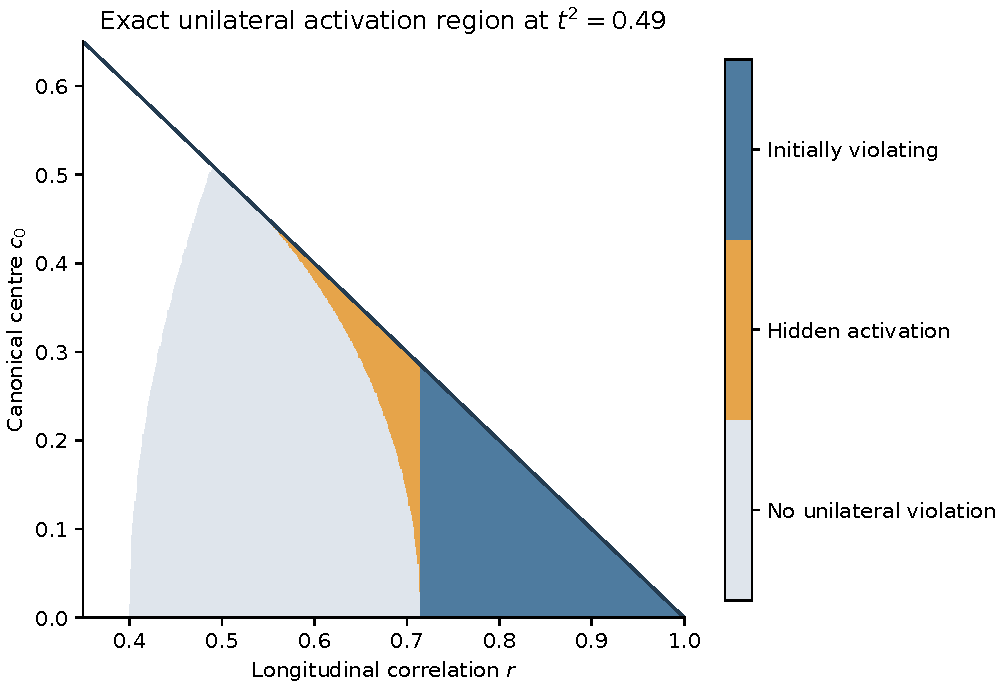
\includegraphics[width=.75\linewidth]{figures/axial_activation_region.pdf}
 \caption{The exact axial activation region at $x=t^2=0.49$.
 The physical region is separated into states with no unilateral
 violation, states with hidden activation, and states that already
 violate CHSH. The boundaries are given by
 \eqref{eq:ext-axial-physical} and~\eqref{eq:ext-axial-activation}.}
 \label{fig:ext-axial-region}
\end{figure}

\begin{corollary}[The quasi-distillable family in the target paper]
\label{cor:ext-quasidistillable}
For
\[
 \rho_p=p|\Psi^-\rangle\langle\Psi^-|
              +(1-p)|00\rangle\langle00|,\qquad 0\le p\le1,
\]
one has
\begin{equation}
 \boxed{\quad
 (B_A^*(\rho_p))^2=(B_B^*(\rho_p))^2
 =\max\left\{1,\frac{2p}{2-p}\right\}.
 \quad}
 \label{eq:ext-quasidistillable}
\end{equation}
For $0<p<2/3$, the value one is a supremum attained only by a
rank-one limit. At and above $p=2/3$, an invertible whitening filter
attains the optimum. At $p=0$, the state is already a pure product.
\end{corollary}

\begin{proof}
For $p>0$, Alice whitening and a local rotation produce the amplitude
damping form $x=r$, $c_0=1-r$, with $r=p/(2-p)$.
The density matrix has rank two, so its boundary value is one.
For $r<1/2$, $\alpha=4r-1<1$, and
Theorem~\ref{thm:ext-threshold} gives exactly one with no finite
attainment. At $r=1/2$, the canonical state already has $B^2=2r=1$.
For $r>1/2$, formula~\eqref{eq:ext-axial-value} has maximum $2r$:
the inequality for the other branch reduces to
$(2r-1)(r-1)\le0$. Symmetry of $\rho_p$ exchanges Alice and Bob.
\end{proof}

This gives a conjecture-free, sharp interval of locally inaccessible hidden
CHSH violation for this family: $0<p\le2/3$.
For comparison, both steering-ellipsoid centres of $\rho_p$ have length
$2(1-p)/(2-p)$, which is at least $1/2$ exactly when $p\le2/3$. Result~1
of~\cite{ducuara} derives the absence of one-sided violation for centre
lengths above $1/2$ from Conjecture~1 of~\cite{milne}, and at centre
length $1/2$ that conjecture also gives $B\le1$; the Omega Institute's
public record of a claimed proof of Conjecture~1~\cite{dossier}
therefore already makes the inaccessibility of $0<p\le2/3$
unconditional, and no priority is claimed for it. What the corollary adds
is the exact value~\eqref{eq:ext-quasidistillable} and the sharpness of the
endpoint: for every $p>2/3$ whitening alone gives a one-sided violation. Indeed, the physical bilateral
filters $F_\varepsilon=\diag(\varepsilon,1)$ on both parties, with
$0<\varepsilon\le1$, produce the same family with parameter and success
probability
\[
 q=\frac{p}{p+(1-p)\varepsilon^2},\qquad
 p_{\rm succ}=p\varepsilon^2+(1-p)\varepsilon^4.
\]
For every $p>0$, $q\to1$ as $\varepsilon\to0$, so the bilateral CHSH supremum
is $\sqrt2$. Directly,
$B(\rho_q)^2=\max\{2q^2,q^2+(1-2q)^2\}$.
For $0<p<1$, the explicit sufficient and necessary condition
$q>1/\sqrt2$ is obtained by choosing
$\varepsilon^2<p(\sqrt2-1)/(1-p)$. Thus every $0<p\le2/3$ permits a
finite-success bilateral violation although neither unilateral filter can
violate. For the exact example $p=3/5$ and $\varepsilon=1/2$, the initial
squared CHSH value is $18/25$, both unilateral suprema have square one,
and the bilateral filtered value has square $72/49$, at success probability
$7/40$. A separate exact rational certificate is included.

The amplitude-damping threshold $r>1/2$ and the loss-channel
golden-ratio threshold are established special cases in
Appendix B of~\cite{zhang}; they are not being claimed as new here.
For example, setting $x=r^2$ and $c_0=1-r$ in
\eqref{eq:ext-axial-activation} gives
$r>(\sqrt5-1)/2$. The theorem supplies one criterion for the full
three-parameter physical family and its exact hidden-activation region.

\section{Success probabilities and an exact constrained dual}
\label{sec:ext-probability}

An optimum conditional CHSH value does not determine a unique success
probability, because a Kraus operator may be scaled down arbitrarily.
Throughout this section, $p_{\max}$ denotes the largest probability
compatible with $F^\dagger F\le I$ for the specified conditional filter.

\begin{proposition}[Exact maximal success probability]
\label{prop:ext-success}
For a canonical effect $I+u\cdot\sigma$,
\begin{equation}
 p_{\max}(0,u)=\frac1{1+\norm u}.
 \label{eq:ext-canonical-success}
\end{equation}
For the original mixed Alice marginal with Bloch vector $a$, the
whitening-and-filtering branch
$F=\sqrt{I+u\cdot\sigma}\,(I+a\cdot\sigma)^{-1/2}$
has
\begin{equation}
 \boxed{
 p_{\max}(a,u)=
 \frac{1-\norm a^2}
 {1-a\cdot u+
 \sqrt{(1-a\cdot u)^2-(1-\norm a^2)(1-\norm u^2)}}.
 }
 \label{eq:ext-original-success}
\end{equation}
\end{proposition}

\begin{proof}
The unscaled branch has success normalization one. If $E=F^\dagger F$,
its largest allowed scalar rescaling has squared size
$1/\lambda_{\max}(E)$, and hence this is its maximum probability.
For a canonical input the effect eigenvalues are $1\pm\norm u$.
For the original state,
\[
 \tr E=\frac{2(1-a\cdot u)}{1-\norm a^2},
 \qquad
 \det E=\frac{1-\norm u^2}{1-\norm a^2}.
\]
The quadratic formula for the larger eigenvalue gives
\eqref{eq:ext-original-success}.
\end{proof}

The next theorem concerns the probability constraint on the
\emph{canonical input}. This restriction is substantive: whitening a
general input changes success probabilities, and
\eqref{eq:ext-original-success}, not~\eqref{eq:ext-canonical-success},
must be used when imposing a probability constraint on the original
state.

\begin{theorem}[One-dimensional convex dual for a success constraint]
\label{thm:ext-success-dual}
Suppose $H_0=K+iC\succ0$, which holds in particular when $\alpha>1$.
Require a canonical filter to have maximum success probability at least
$p_0\in[1/2,1]$, and put
$R=p_0^{-1}-1\in[0,1]$.
Let $S_R$ be the largest squared CHSH value under that constraint.
Then
\begin{equation}
 \boxed{
 S_R=\inf_{\tau\ge0}
 \left[
 \tr A+\tau R^2
 -\lambda_{\min}\!\left(A+C(K+\tau I)^{-1}C\right)
 \right].
 }
 \label{eq:ext-success-dual}
\end{equation}
The function minimized is convex in $\tau$.
For $R>0$ it has a finite minimizer, and a corresponding optimal
filter can be reconstructed from its minimum eigenspace.
The value is nondecreasing and concave as a function of $R^2$.
It reaches the unconstrained plateau at
\begin{equation}
 R_*^2=
 \min_{\substack{\norm n=1\\Mn=\lambda_{\min}(M)n}}
       \norm{K^{-1}Cn}^2.
 \label{eq:ext-plateau-radius}
\end{equation}
At $R=0$, $S_0=\tr A-\lambda_{\min}(A)$ is the original canonical
CHSH value.
\end{theorem}

\begin{proof}
The probability constraint is exactly $\norm u\le R$.
The Lorentz reduction in the proof of the main theorem respects it.
Indeed its replacement filter has squared effect norm
$1-1/\Delta$, whereas the original filter has squared effect norm
$1-1/w_0^2$, and $\Delta\le w_0^2$.
Thus replacement decreases the norm and cannot lower the chosen
correlation-plane value. Conversely each reduced feasible pair gives
$u=-n\times v$ with $\norm u=\norm v$.
It follows that $S_R$ is exactly the maximum of $f(n,v)$ subject to
$\norm n=1$, $n\cdot v=0$, and $\norm v\le R$.

For $\tau\ge0$, write
$P_\tau=K+\tau I$ and $M_\tau=A+CP_\tau^{-1}C$.
Completing the square gives, for every feasible pair,
\begin{align}
 f(n,v)
 ={}&\tr A-n^TM_\tau n+\tau\norm v^2 \notag\\
    &-(v+P_\tau^{-1}Cn)^TP_\tau
                  (v+P_\tau^{-1}Cn)
 \le\tr A+\tau R^2-\lambda_{\min}(M_\tau).
 \label{eq:ext-dual-square}
\end{align}
This proves weak duality. The expression on the right is also the
maximum, over $\norm n=1$ and arbitrary real $v$, of
$f(n,v)+\tau(R^2-\norm v^2)$, with the orthogonality constraint
temporarily omitted. It is therefore a supremum of affine functions
of $\tau$, and is convex. For $R>0$ it tends to infinity as
$\tau\to\infty$, so it has a minimizer.

Let $N_\tau$ have orthonormal columns spanning the minimum eigenspace
of $M_\tau$.
The possible squared norms of
$v=-P_\tau^{-1}Cn$, for unit $n$ in that eigenspace, form the whole
Rayleigh interval
\begin{equation}
 [r_-^2(\tau),r_+^2(\tau)]
 =\left[
 \lambda_{\min}(N_\tau^TC^TP_\tau^{-2}CN_\tau),
 \lambda_{\max}(N_\tau^TC^TP_\tau^{-2}CN_\tau)
 \right].
 \label{eq:ext-radius-interval}
\end{equation}
Here $M_\tau'=-CP_\tau^{-2}C=C^TP_\tau^{-2}C$.
The left and right derivatives of the convex dual function are
$R^2-r_+^2(\tau)$ and $R^2-r_-^2(\tau)$, respectively.
At a positive minimizing $\tau$, they bracket zero, so choose a unit
minimum eigenvector whose associated $v$ has norm exactly $R$.
At a minimizer $\tau=0$, the right derivative is nonnegative,
so choose one with $\norm v\le R$.

It remains to check the omitted orthogonality condition.
The positive matrix $H_0+\tau I=P_\tau+iC$ has Schur complement
\[
 P_\tau+CP_\tau^{-1}C
 =M_\tau+(\tau-s)I\succ0.
\]
The paired eigenvector equations therefore force
$(\lambda_{\min}(M_\tau)+\tau-s)n\cdot v=0$ with a strictly
positive coefficient, so $n\cdot v=0$.
The selected pair is feasible and gives equality in
\eqref{eq:ext-dual-square}, proving strong duality.
This argument uses the entire eigenspace and therefore includes
eigenvalue crossings.

The infimum of affine functions of $R^2$ is concave; monotonicity
also follows directly from nesting of the feasible balls.
At $\tau=0$, the same one-sided derivative test is precisely
$R^2\ge R_*^2$, proving the plateau assertion.
For $R=0$, the primal domain forces $v=0$, and the dual tends to
the same value as $\tau\to\infty$.
\end{proof}

Equation~\eqref{eq:ext-success-dual} is an exact convex scalar
representation. In general it is not asserted to be a formula in
radicals. The axial family does permit a complete piecewise expression,
including an interval where the best filter breaks the apparent axial
symmetry.

\begin{theorem}[Closed axial frontier and tilted optimal filters]
\label{thm:ext-axial-frontier}
For~\eqref{eq:ext-axial-family}, suppose $H_0\succ0$, and put
\[
 k=x-c_0^2,\qquad g=rc_0>0,\qquad R_*=\frac gk<1.
\]
If $x\le r^2$, then
\begin{equation}
 S_R=
 \begin{cases}
  x+r^2+2gR-kR^2,&0\le R\le R_*,\\
  x+r^2+g^2/k,&R\ge R_*.
 \end{cases}
 \label{eq:ext-axial-frontier-first}
\end{equation}
If $x>r^2$ and $g^2\le k(x-r^2)$, then $S_R=2x$ for every $R$.
In the remaining case, define
\[
 \tau_c=\frac{g^2}{x-r^2}-k>0,\qquad
 R_c=\frac{x-r^2}{g},\qquad 0<R_c<R_*.
\]
Then
\begin{equation}
 \boxed{
 S_R=
 \begin{cases}
 2x+\tau_cR^2,&0\le R\le R_c,\\
 x+r^2+2gR-kR^2,&R_c\le R\le R_*,\\
 x+r^2+g^2/k,&R\ge R_*.
 \end{cases}}
 \label{eq:ext-axial-frontier}
\end{equation}
For $0<R<R_c$, one optimal effect is
\begin{equation}
 u=\left(-R\sqrt{1-(R/R_c)^2},\,0,\,R^2/R_c\right),
 \label{eq:ext-tilted-effect}
\end{equation}
up to rotations about the symmetry axis. Every optimal effect in this
open interval has a nonzero component perpendicular to that axis.
For $R_c\le R\le R_*$, an optimal effect is $u=(0,0,R)$; above
the plateau, replace $R$ by $R_*$.
\end{theorem}

\begin{proof}
Positivity of $H_0$ is equivalent here to $k>g$ and $r^2>c_0^2$.
The eigenvalues of $M_\tau$ are
$x-g^2/(k+\tau)$, twice, and $r^2$.
Consequently the dual objective is the \emph{upper} envelope
\begin{equation}
 \max\left\{
 x+r^2+\tau R^2+\frac{g^2}{k+\tau},\
 2x+\tau R^2
 \right\}.
 \label{eq:ext-axial-dual-envelope}
\end{equation}
If $x\le r^2$, the first branch is always active. Its minimizing
parameter for $R>0$ is $\tau=\max(g/R-k,0)$, yielding
\eqref{eq:ext-axial-frontier-first}; at $R=0$ the infimum is
obtained as $\tau\to\infty$.
If $x>r^2$ but $\tau_c\le0$, the second branch is always active,
and $\tau=0$ gives the constant value $2x$.

In the remaining case the first branch applies for
$0\le\tau\le\tau_c$, and the second for $\tau\ge\tau_c$.
For $0<R<R_c$ their left and right slopes at the crossing have
opposite signs, so the minimum is at $\tau_c$.
At $R=0$, every $\tau\ge\tau_c$ has the minimum value $2x$.
For $R_c\le R\le R_*$ it is at $\tau=g/R-k$;
for $R\ge R_*$ it is at zero. Substitution proves all three pieces.

At $\tau_c$, the minimum eigenspace is all of $\R^3$.
Set $\theta=(R/R_c)^2$ and choose
\[
 n=(\sqrt\theta,0,\sqrt{1-\theta}),\qquad
 v=(0,-R_c\sqrt\theta,0).
\]
These vectors satisfy $\norm n=1$, $n\cdot v=0$, and $\norm v=R$,
and give~\eqref{eq:ext-tilted-effect}.
Moreover every equality pair must have
$v=-(K+\tau_cI)^{-1}Cn$ and $\norm v=R$.
It follows that the transverse squared norm of $n$ is $\theta$,
so $\norm{u_\perp}=R\sqrt{1-\theta}>0$.
Thus a restriction to axial effects loses the true optimum throughout
this interval.
\end{proof}

\subsection{An exact probability threshold inside the tilted regime}

Return to the canonical activation example
$\rho_1=\tfrac1{40}\left(\begin{smallmatrix}
20&0&0&14\\0&0&0&0\\0&0&7&0\\14&0&0&13
\end{smallmatrix}\right)$ from the earlier examples.
Here
\[
 x=\frac{49}{100},\quad r=\frac{13}{20},\quad c_0=\frac7{20},
 \quad k=\frac{147}{400},\quad g=\frac{91}{400}.
\]
The exact breakpoints and scalar dual parameter are
\[
 R_c=\frac{27}{91},\qquad
 R_*=\frac{13}{21},\qquad
 \tau_c=\frac{539}{1350}.
\]
Thus
\begin{equation}
 S_R=
 \begin{cases}
 \displaystyle\frac{49}{50}+\frac{539}{1350}R^2,
       &0\le R\le27/91,\\[3pt]
 \displaystyle\frac{73}{80}+\frac{91}{200}R-\frac{147}{400}R^2,
       &27/91\le R\le13/21,\\[3pt]
 \displaystyle\frac{79}{75},&R\ge13/21.
 \end{cases}
 \label{eq:ext-exact-frontier}
\end{equation}
The constrained state violates CHSH exactly when
\begin{equation}
 R>\sqrt{\frac{27}{539}}
 \quad\Longleftrightarrow\quad
 p_0<\frac1{1+\sqrt{27/539}}.
 \label{eq:ext-success-threshold}
\end{equation}
Since $\sqrt{27/539}<27/91$, the first onset of violation occurs
strictly inside the tilted-filter regime. This is a concrete obstruction
to optimizing the success tradeoff by assuming that an axially symmetric
input has an axial optimal filter.

\begin{figure}[tbp]
 \centering
 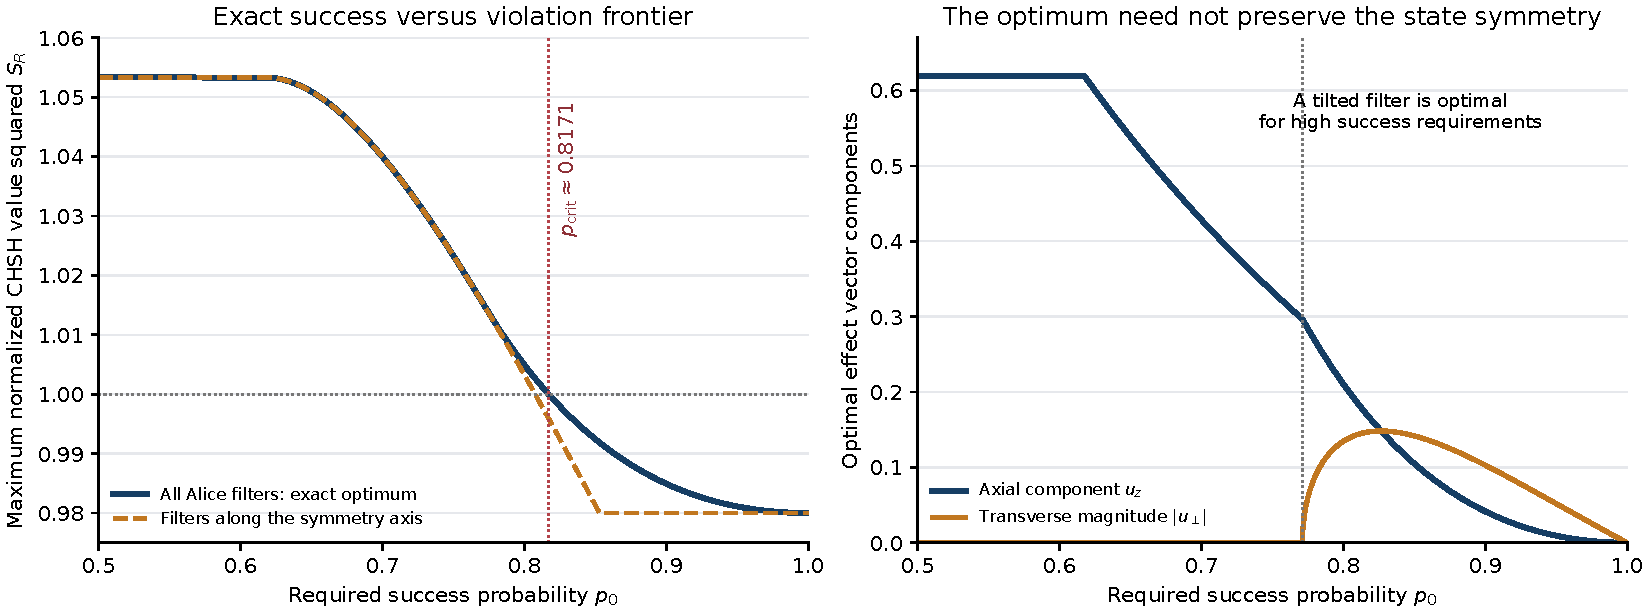
\includegraphics[width=\linewidth]{figures/exact_success_frontier.pdf}
 \caption{The exact success frontier for $\rho_1$.
 Left: the unrestricted optimum~\eqref{eq:ext-exact-frontier}
 compared with filters constrained to the symmetry axis.
 Right: the axial and transverse components of an optimal effect.
 A nonzero transverse component is necessary throughout the high-success
 interval corresponding to $0<R<R_c$.}
 \label{fig:ext-success-frontier}
\end{figure}


\section{Success constraints on the original input state}
\label{sec:r3-success}

The earlier scalar dual constrains the success probability on a canonical
input. Whitening is itself probabilistic, so that dual does not directly
solve the tradeoff on the original state. This section gives the correct
feasible geometry, an exact algebraic optimization for every input, and
closed frontiers for several noncanonical families.

Let the original Alice marginal have Bloch vector $a$, with
$r=\norm a<1$, and put $W=(I+a\cdot\sigma)^{-1/2}$.
Write the canonical data as $(c,D)$ and set $Q=D^TD$.
For $0\le p\le1$, define
\[
 S_\rho(p)=
 \sup_{\substack{F\text{ invertible},\ F^\dagger F\preceq I\\
                  \tr[(F^\dagger F\otimes I)\rho]\ge p}}
 B(\rho_F)^2.
\]
Thus $p$ is a required success probability, rather than the probability
of a particular arbitrarily rescaled Kraus operator.

\subsection{Two balls, rather than a centered-radius constraint}

\begin{theorem}[Exact original-input success lens]
\label{thm:r3-lens}
A canonical effect vector $u$, $\norm u\le1$, can be implemented on the
original state with success probability at least $p$ if and only if
\begin{equation}
 \boxed{\qquad \norm{a-pu}\le1-p.\qquad}
 \label{eq:r3-lens}
\end{equation}
Consequently its feasible set is
\begin{equation}
 \mathcal L_p(a)=
 \{u:\norm u\le1,\ \norm{a-pu}\le1-p\}.
 \label{eq:r3-lens-set}
\end{equation}
For $p>0$, the second condition is the ball centered at $a/p$ of
radius $(1-p)/p$. The constraint is inactive when
$p\le(1-r)/2$. That second ball lies inside the unit ball when
$p\ge(1+r)/2$. At $p=1$ the lens is the singleton $\{a\}$.

The smallest and largest feasible norms are
\begin{equation}
 r_-(p)=\max\left\{0,1-\frac{1-r}{p}\right\},\qquad
 r_+(p)=\min\left\{1,\frac{1+r}{p}-1\right\},
 \label{eq:r3-radius-range}
\end{equation}
with $r_-(0)=0$ and $r_+(0)=1$.
\end{theorem}

\begin{proof}
The unscaled combined filter is
$F_u=\sqrt{I+u\cdot\sigma}\,W$, and its success normalization on
$\rho$ is one. Its largest physical success probability is
$1/\lambda_{\max}(E_u)$, where
$E_u=W(I+u\cdot\sigma)W$. Hence success at least $p$ is equivalent to
$pE_u\preceq I$. Congruence by $W^{-1}$ turns this into
\[
 p(I+u\cdot\sigma)\preceq I+a\cdot\sigma.
\]
The difference has eigenvalues $1-p\pm\norm{a-pu}$, proving
\eqref{eq:r3-lens}.
The two ball-containment conditions follow by comparing their center
distance $r/p$ and radii $1,(1-p)/p$.

The nearest point of the second ball to the origin has distance
$\max(0,[r-(1-p)]/p)=r_-(p)$, and it lies in the unit ball since
$r_-(p)\le r<1$.
The farthest feasible distance is the smaller of one and the second
ball's farthest distance $(r+1-p)/p$.
Both extrema are obtained on the line through $a$; if $a=0$, any
radial direction may be used for the maximum.
\end{proof}

In particular, whitening $u=0$ is allowed exactly when $p\le1-r$,
which is a different threshold from the condition that \emph{every}
canonical filter is allowed.

\begin{figure}[htbp]
\centering
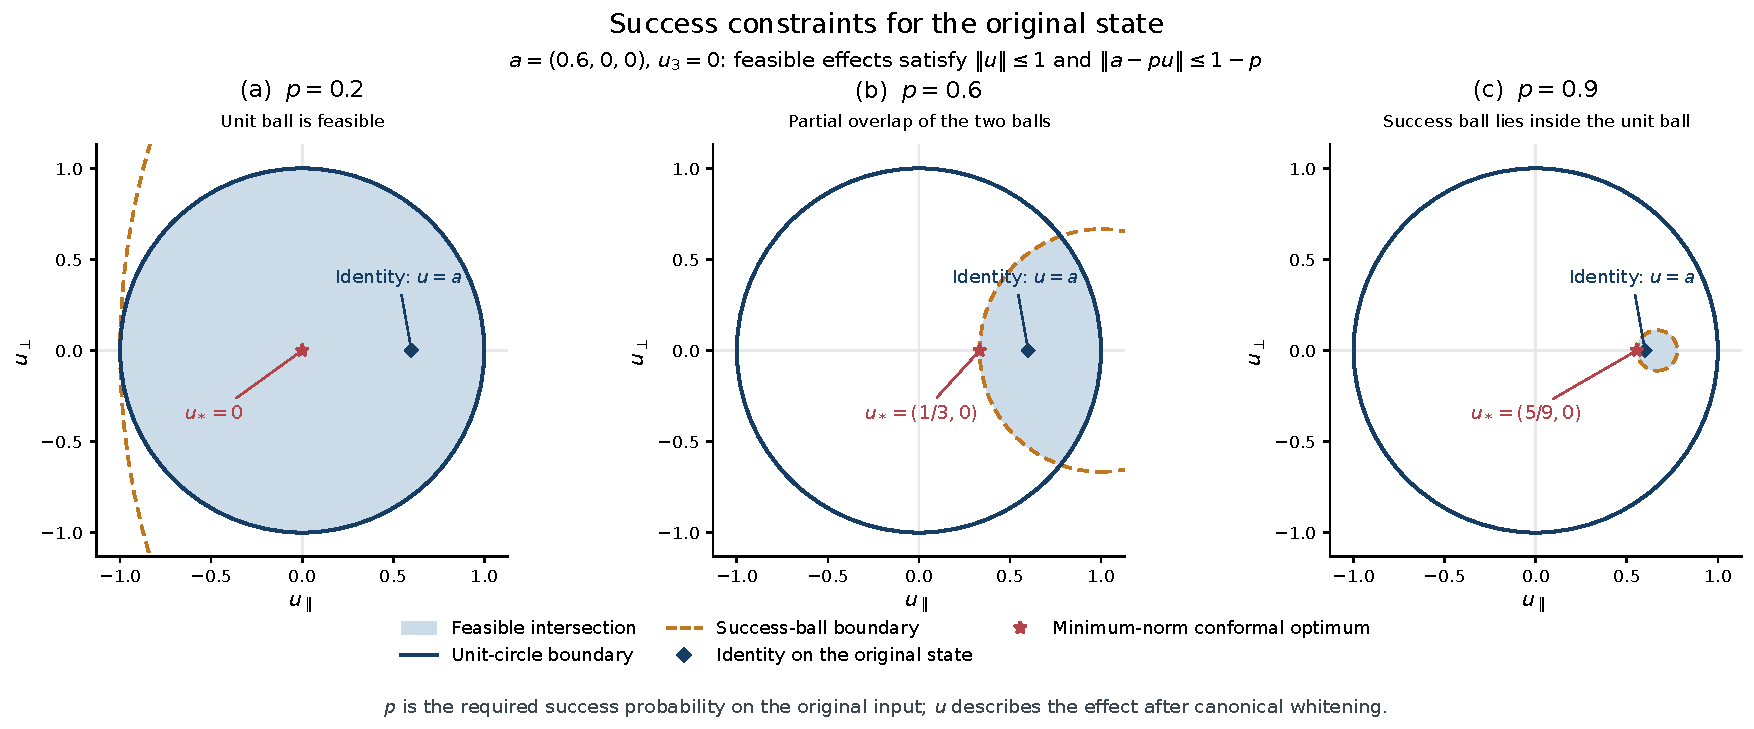
\includegraphics[width=\textwidth]{figures/original_success_lens.pdf}
\caption{Planar sections of the exact original-input success lens at
$\norm a=0.6$. As the required probability increases, the feasible region
changes from the entire effect ball to a lens and then to a smaller ball.
The identity filter on the original state corresponds to $u=a$ and remains
feasible. The closest point to the origin
is the exact optimum for the conformal family of Theorem~\ref{thm:r3-conformal}.}
\label{fig:r3-lens}
\end{figure}

\begin{lemma}[Density of invertible filters and attainment above one]
\label{lem:r3-density}
Maximizing a continuous filtered score over the closed lens gives the
same value as the invertible-filter supremum.
Every constrained optimum with $S_\rho(p)>1$ is attained by an
invertible filter.
\end{lemma}

\begin{proof}
For $p<1$, the point $u=a$ is strictly inside both defining balls:
$\norm a<1$ and $\norm{a-pa}=(1-p)r<1-p$.
For any feasible $u$, the points $u_t=(1-t)u+ta$, $0<t\le1$,
remain feasible by convexity and satisfy $\norm{u_t}<1$.
They converge to $u$, so invertible effects are dense.
At $p=1$, the only feasible point is already the interior point $a$.
Finally, $\norm u=1$ gives a rank-one Alice filter and therefore a
product output, whose normalized CHSH value is at most one.
A compact maximizer with value greater than one must consequently
have $\norm u<1$.
\end{proof}

\subsection{The correct quadratic Gram matrix}

\begin{theorem}[An exact three-variable constrained optimization]
\label{thm:r3-gram}
Define the polynomial symmetric matrix
\begin{equation}
 \boxed{
 G(u)=(1-\norm u^2)(Q-cc^T)
             +(c+D^Tu)(c+D^Tu)^T.
 }
 \label{eq:r3-bob-gram}
\end{equation}
Then, for every canonical effect including $\norm u=1$,
$G(u)=T_u^TT_u$. In particular
\begin{equation}
 \boxed{
 S_\rho(p)=\max_{u\in\mathcal L_p(a)}
       [\,\tr G(u)-\lambda_{\min}(G(u))\,].
 }
 \label{eq:r3-primal}
\end{equation}
Equivalently, for each unit Bob-side normal $n$, put $P_n=I-nn^T$,
\[
 k_n=\tr[P_n(Q-cc^T)],\qquad
 h_n=DP_nc,\qquad J_n=k_nI-DP_nD^T.
\]
The objective associated with that measurement plane is the quadratic
\begin{equation}
 f_n(u)=\tr(P_nQ)+2h_n^Tu-u^TJ_nu,
 \qquad
 S_\rho(p)=\max_{\norm n=1}\max_{u\in\mathcal L_p(a)}f_n(u).
 \label{eq:r3-plane-quadratic}
\end{equation}
\end{theorem}

\begin{proof}
Set $q=\sqrt{1-\norm u^2}$ and
$S_u=qI+uu^T/(1+q)$.
The filtered correlation matrix is $T_u=S_uD+uc^T$.
The identities $S_uu=u$ and $S_u^2=(1-\norm u^2)I+uu^T$
give
\[
 T_u^TT_u=(1-\norm u^2)Q
  +(D^Tu)(D^Tu)^T+(D^Tu)c^T+c(D^Tu)^T+\norm u^2cc^T,
\]
which is~\eqref{eq:r3-bob-gram}. This calculation remains valid at
the rank-one boundary. The Horodecki formula gives
\eqref{eq:r3-primal}; compactness and
Lemma~\ref{lem:r3-density} justify the maximum.
Taking $\tr(P_nG(u))$ and expanding proves
\eqref{eq:r3-plane-quadratic}.
\end{proof}

The Bob-side normal in~\eqref{eq:r3-plane-quadratic} is unrestricted.
It must not be constrained to be perpendicular to $u$.
The Lorentz replacement in the unconstrained proof can change the
effect vector toward the origin, which need not preserve a ball centered
at $a/p$.

\begin{remark}[An exact counterexample to the naive shifted reduction]
\label{rem:r3-counterexample}
Take the full-rank original state
\begin{equation}
 \rho=\frac1{200}
 \begin{pmatrix}
 116&0&0&56\\0&44&8&0\\0&8&11&0\\56&0&0&29
 \end{pmatrix}.
 \label{eq:r3-counterexample}
\end{equation}
The two block determinants before division by $200^2$ are $228$ and
$420$, so positivity is strict. Here $a=(0,0,3/5)$, and the canonical
data are $c=0$, $D=\diag(4/5,-3/5,9/20)$.
Thus $K=DD^T\succ0$ and $\alpha=481/400>1$.
At $p=1$, only $u=a$ is feasible, and the true score is
$S_\rho(1)=16/25$.
If one instead imposes $u=-n\times v=a$ in the earlier reduced
objective, one forces $n\perp a$ and obtains only
\[
 (16/25)^2+(9/20)^2=\frac{6121}{10000}
 <\frac{16}{25}.
\]
The failure therefore occurs even inside the positive-Gram regime.
\end{remark}

\subsection{A rational description using the ellipsoid and original marginals}

\begin{theorem}[The full frontier needs no canonical orientation]
\label{thm:r3-ellipsoid}
Let $b$ be the original Bob Bloch vector, $g=b-c=D^Ta$, and
$Q=D^TD$. If $Q\succ0$, set $w=D^Tu$. Then the exact frontier is
obtained by maximizing the top-two eigenvalue sum of
\begin{equation}
 \mathcal G(w)=
 (1-w^TQ^{-1}w)(Q-cc^T)+(c+w)(c+w)^T
 \label{eq:r3-ellipsoid-gram}
\end{equation}
under the two ellipsoid constraints
\begin{equation}
 w^TQ^{-1}w\le1,\qquad
 (g-pw)^TQ^{-1}(g-pw)\le(1-p)^2.
 \label{eq:r3-two-ellipsoids}
\end{equation}
All coefficients are rational functions of the original Bloch data.

The same statement extends to singular $Q$ as follows.
Write $Q^\dagger$ for its Moore--Penrose inverse, restrict
$w\in\ran Q$, and put
\[
 \eta=\norm a^2-g^TQ^\dagger g\ge0.
\]
If $\rank Q<3$ and $\eta>0$, introduce $k\ge0$ and set
\begin{align}
 q&=w^TQ^\dagger w+k^2/\eta,\\
 \ell&=(g-pw)^TQ^\dagger(g-pw)
              +\eta-2pk+p^2k^2/\eta.
 \label{eq:r3-singular-positive}
\end{align}
If $\rank Q<3$ and $\eta=0$, introduce $t\ge0$ and instead set
\begin{equation}
 q=w^TQ^\dagger w+t,\qquad
 \ell=(g-pw)^TQ^\dagger(g-pw)+p^2t.
 \label{eq:r3-singular-zero}
\end{equation}
In both cases maximize the top-two eigenvalue sum of
\begin{equation}
 (1-q)(Q-cc^T)+(c+w)(c+w)^T
 \label{eq:r3-singular-gram}
\end{equation}
under $q\le1$ and $\ell\le(1-p)^2$.
This is exact, including all rank-zero, rank-one, and rank-two shapes.
After choosing coordinates in $\ran Q$, it uses at most three real
variables and has rational coefficients on each rank stratum.
\end{theorem}

\begin{proof}
When $D$ is invertible, $u=D^{-T}w$ and $a=D^{-T}g$, proving
\eqref{eq:r3-two-ellipsoids} and~\eqref{eq:r3-ellipsoid-gram}.
The equality $g=b-c$ follows by applying the effect $u=a$, which
undoes whitening and restores the original Bob marginal.
Alternatively it follows directly from
$c=(b-T^Ta)/(1-\norm a^2)$.

For the singular case decompose orthogonally
\[
 u=DQ^\dagger w+u_0,\qquad
 a=DQ^\dagger g+a_0,\qquad
 u_0,a_0\in\ker D^T.
\]
Then $\norm{a_0}^2=\eta$ and
$\norm u^2=w^TQ^\dagger w+\norm{u_0}^2$.
The Gram matrix depends on $u_0$ only through its squared norm.
For a fixed norm, the smallest possible value of
$\norm{a_0-pu_0}^2$ is obtained by aligning $u_0$ with $a_0$.
If $\eta>0$, write $u_0=(k/\eta)a_0$ with $k\ge0$.
Its norm and distance are exactly the extra terms
in~\eqref{eq:r3-singular-positive}.
If $\eta=0$, choose any null-space vector of squared norm $t$,
giving~\eqref{eq:r3-singular-zero}.
This alignment preserves the score and can only improve success
feasibility; every reduced feasible point reconstructs a real filter.

The raw formulas for $c,Q$ are rational, as in
\eqref{eq:ext-raw-ellipsoid}. The pseudoinverse is rational on each
rank stratum. Explicitly, with $e_1=\tr Q$ and
$e_2=((\tr Q)^2-\tr Q^2)/2$,
\[
 Q^\dagger=
 \begin{cases}
 0,&\rank Q=0,\\
 Q/e_1^2,&\rank Q=1,\\
 [(e_1^2-e_2)Q-e_1Q^2]/e_2^2,&\rank Q=2,\\
 \adj(Q)/\det Q,&\rank Q=3.
 \end{cases}
\]
Each formula follows by evaluation on the nonzero eigenvalues.
For rank below three, there are $\rank Q$ range coordinates and one
additional scalar, proving the dimension bound.
\end{proof}

This theorem says precisely which extra data the original-input
tradeoff needs: the steering ellipsoid $(Q,c)$, the original Bob point
$b$, and the length $\norm a$. In the nonsingular case the latter is
already encoded by $g^TQ^{-1}g$.
The conditional Bob Bloch vector is $c+w$; the second ellipsoid
constraint is the condition that the complementary outcome can also
have a conditional Bob vector in the same ellipsoid.

\subsection{Exact algebraic decisions and verifiable upper certificates}

\begin{proposition}[Degree-six decision and a complete certificate hierarchy]
\label{prop:r3-certificates}
For a proposed squared-score threshold $\gamma$, define
\[
 H_\gamma(u)=\gamma I-\tr G(u)I+G(u),\quad
 g_1(u)=1-\norm u^2,\quad
 g_2(u)=(1-p)^2-\norm{a-pu}^2.
\]
Then $S_\rho(p)>\gamma$ exactly when there is a real $u$ with
$g_1,g_2\ge0$ for which at least one of
\begin{equation}
 \tr H_\gamma,\qquad
 \frac{(\tr H_\gamma)^2-\tr(H_\gamma^2)}2,\qquad
 \det H_\gamma
 \label{eq:r3-polynomial-decision}
\end{equation}
is negative. These are polynomials of degree at most $2,4,6$ in
the three coordinates of $u$. Thus real quantifier elimination gives
an exact algebraic decision for algebraic input data.

An exact polynomial identity
\begin{equation}
 H_\gamma=\Sigma_0+g_1\Sigma_1+g_2\Sigma_2,
 \qquad \Sigma_j=\sum_\ell V_{j\ell}^TV_{j\ell},
 \label{eq:r3-sos-certificate}
\end{equation}
is a sufficient upper certificate $S_\rho(p)\le\gamma$.
For every strict upper threshold $\gamma>S_\rho(p)$, such a
matrix sum-of-squares certificate exists at some finite degree.
\end{proposition}

\begin{proof}
The largest eigenvalue of $\tr G\,I-G$ is the sum of the two largest
eigenvalues of $G$. Thus $H_\gamma\succeq0$ is exactly the
pointwise upper-score condition. The three elementary symmetric
coefficient test for a real symmetric $3\times3$ matrix proves
\eqref{eq:r3-polynomial-decision}; the degree bounds follow because
$G$ is quadratic in $u$.

Every right-hand term in~\eqref{eq:r3-sos-certificate} is positive
semidefinite on the lens, proving sufficiency by direct evaluation.
For completeness, if $\gamma>S_\rho(p)$, then $H_\gamma$ is
uniformly positive definite on the compact lens.
The matrix Positivstellensatz of Hol--Scherer~\cite{holscherer2005}
applies: the quadratic module is Archimedean because it already
contains $1-\norm u^2$.
It supplies the displayed representation. No fixed degree is asserted,
and at equality $\gamma=S_\rho(p)$ finite-degree attainment is not
guaranteed.
\end{proof}

Thus one may search for upper certificates by semidefinite programming,
but floating-point feasibility alone is not a certificate: the
polynomial identity and the positive semidefinite Gram matrices must
be checked exactly or with rigorous error bounds. Likewise, the
general-purpose multistart optimizer supplied with this report only
produces numerical candidates. It is not an exact replacement for
quantifier elimination or a verified certificate.

There is additional convex structure for a \emph{fixed} Bob plane.
If $K\succ0$, then $J_n\succ0$ for every $n$: the two nonzero
eigenvalues of $DP_nD^T$ are those of $Q$ restricted to the plane,
so its largest eigenvalue subtracted from $k_n$ leaves at least
$\lambda_{\min}(Q)-\norm c^2>0$.
For $p<1$, strict feasibility at $u=a$ gives the exact inner dual
\begin{align}
 \max_{u\in\mathcal L_p(a)} f_n(u)
 =\min_{\lambda,\mu\ge0}\bigl\{
 &\tr(P_nQ)+\lambda+\mu[(1-p)^2-r^2]\notag\\
 &+(h_n+\mu p a)^T
 [J_n+(\lambda+\mu p^2)I]^{-1}
 (h_n+\mu p a)\bigr\}.
 \label{eq:r3-fixed-plane-dual}
\end{align}
This follows by completing the square and the ordinary strictly
feasible concave quadratic-program duality theorem.
It does not justify interchanging the outer maximum over $n$ with
the dual minimum. No universal scalar dual for the original-state
frontier is claimed here.

\subsection{Universal purity bounds and exact closed families}

Let $\alpha=\tr(DD^T)-\norm c^2$ and $m=(\alpha-1)/2$.
For clarity, the pointwise inequality needed here concerns the
\emph{actual effect} $u$, without any replacement by a reduced
Lorentz pair:
\begin{equation}
 B((\rho_c)_u)^2\le 1+m(1-\norm u^2).
 \label{eq:r3-pointwise-purity}
\end{equation}
One direct proof is as follows. For an arbitrary physical state
$\omega$ with Bloch data $(a',b',T')$, a real unit vector $n$, and
$S_n=(n\cdot\sigma)\otimes I$, Pauli orthogonality gives
\begin{align*}
 4\tr(\omega S_n\widetilde\omega S_n)
 ={}&1+\norm{a'}^2-\norm{b'}^2-\norm{T'}_F^2\\
 &-2(n\cdot a')^2+2n^TT'T'^Tn\ge0.
\end{align*}
The inequality holds because both $\omega$ and
$S_n\widetilde\omega S_n$ are positive semidefinite. Therefore each
Alice measurement-plane score satisfies
\[
 \tr(T'T'^T)-n^TT'T'^Tn
 \le\frac{1+\norm{T'}_F^2+\norm{a'}^2-\norm{b'}^2}{2}
       -(n\cdot a')^2.
\]
For the actual canonical effect, $a'=u$, $b'=c+D^Tu$, and
\eqref{eq:r3-bob-gram} gives
\[
 \norm{T'}_F^2+\norm u^2-\norm{b'}^2
   =\alpha+(1-\alpha)\norm u^2.
\]
Taking the maximum over measurement planes and dropping the
nonnegative square proves~\eqref{eq:r3-pointwise-purity}, including
$\norm u=1$. This is the quantitative purity bound from
Proposition~\ref{prop:ext-purity}, now written entirely in the
coordinates of the constrained problem.

Combining it with the exact norm range of the lens yields
\begin{equation}
 S_\rho(p)\le
 \begin{cases}
 1+m[1-r_-(p)^2],&m\ge0,\\
 1+m[1-r_+(p)^2],&m<0.
 \end{cases}
 \label{eq:r3-purity-frontier}
\end{equation}
The following families attain either this bound or a sharper exact
spectral expression. Their proofs optimize over all filter directions.

\begin{theorem}[Conformal canonical correlations: full-rank and pure frontiers]
\label{thm:r3-conformal}
Suppose the canonical state is physical and has $c=0$, $D=tO$,
where $t\ge0$ and $O$ is orthogonal. Then
\begin{equation}
 \boxed{\qquad S_\rho(p)=t^2[\,2-r_-(p)^2\,].\qquad}
 \label{eq:r3-conformal}
\end{equation}
For $t>0$, the optimal canonical effect is uniquely
$u_*=r_-(p)a/r$ when $r>0$, and $u_*=0$ when $r=0$.
All these optima are attained by invertible filters.
The plateau extends to $p=1-r$.
This includes arbitrary one-sided invertible-filter images of the
Werner/isotropic canonical family, and includes every entangled pure
state at $t=1$.
\end{theorem}

\begin{proof}
Here $G(u)=t^2[(1-\norm u^2)I+O^Tuu^TO]$.
Its eigenvalues are $t^2$, $t^2(1-\norm u^2)$, and
$t^2(1-\norm u^2)$. The score is therefore
$t^2(2-\norm u^2)$, so its maximum is reached at the unique
minimum-norm point of the lens when $t>0$.
The minimum norm is $r_-(p)\le r<1$, proving finite attainment.
An entangled pure state becomes maximally entangled after whitening,
which gives $t=1$.
\end{proof}

An explicit largest-scale filter on the \emph{original} state is
especially simple. In the eigenbasis of $\rho_A$, with the larger
eigenvalue first, use
\begin{equation}
 F_p=
 \begin{cases}
 \diag\!\left(\sqrt{\dfrac{1-r}{1+r}},1\right),&p\le1-r,\\[6pt]
 \diag\!\left(\sqrt{\dfrac{2p-1+r}{1+r}},1\right),&p\ge1-r.
 \end{cases}
 \label{eq:r3-concentration-filter}
\end{equation}
The first branch succeeds with probability $1-r$, and the second
with probability exactly $p$. Both are continuous at the breakpoint.
For $r=0$, this prescription is simply the identity.

\begin{corollary}[Exact original-input threshold for the full-rank example]
\label{cor:r3-rho2}
For
\[
 \rho_2=\frac1{500}
 \begin{pmatrix}
 441&0&0&56\\0&49&0&0\\0&0&1&0\\56&0&0&9
 \end{pmatrix},
\]
the canonical parameters are $t=4/5$, $r=24/25$. Hence
\begin{equation}
 S_{\rho_2}(p)=\frac{16}{25}
 \left[2-\max\left(0,1-\frac1{25p}\right)^2\right],
 \label{eq:r3-rho2-frontier}
\end{equation}
with the maximum taken as zero inside the square at $p=0$.
The maximal CHSH score is available up to success $1/25$,
whereas some violation is available exactly when
\begin{equation}
 \boxed{\qquad
 p<\frac{4(4+\sqrt7)}{225}\simeq0.11815.
 \qquad}
 \label{eq:r3-rho2-threshold}
\end{equation}
\end{corollary}

\begin{proof}
The first statement follows from~\eqref{eq:r3-conformal}.
Above the plateau, violation is
$1-1/(25p)<\sqrt{2-25/16}=\sqrt7/4$.
Solving and rationalizing its positive denominator yields
\eqref{eq:r3-rho2-threshold}. At equality the squared score is one.
\end{proof}

\begin{theorem}[Arbitrary maximally correlated rank-two states]
\label{thm:r3-correlated}
For
\[
 \rho_{v,z}=v|00\rangle\langle00|+(1-v)|11\rangle\langle11|
       +z|00\rangle\langle11|+\overline z|11\rangle\langle00|,
 \quad 0<v<1,\quad |z|^2\le v(1-v),
\]
put $r=|2v-1|$ and $t^2=|z|^2/[v(1-v)]$. Then
\begin{equation}
 \boxed{\qquad
 S_{\rho_{v,z}}(p)=1+t^2[1-r_-(p)^2].
 \qquad}
 \label{eq:r3-correlated}
\end{equation}
The original-state filter~\eqref{eq:r3-concentration-filter} attains
the optimum. For $z\ne0$ its positive part is unique up to scale.
\end{theorem}

\begin{proof}
A phase rotation makes $z$ nonnegative. Whitening gives $c=0$ and,
with the perfect-correlation direction chosen as the third axis,
$D=\diag(t,-t,1)$.
Here $m=t^2$, so~\eqref{eq:r3-purity-frontier} is precisely the
claimed upper bound. The vector $a$ is on the perfect-correlation
axis. At the closest feasible effect $u=(0,0,\pm r_-(p))$,
the Gram eigenvalues are
$1,t^2(1-r_-(p)^2),t^2(1-r_-(p)^2)$, giving equality.
The filter in~\eqref{eq:r3-concentration-filter} realizes this
effect. If $t>0$, equality in the upper bound requires the unique
minimum-norm point of the lens, proving uniqueness.
\end{proof}

\begin{theorem}[All product states, including pure marginals]
\label{thm:r3-product}
For $\rho=\rho_A\otimes\rho_B$, let $r=\norm a$ and $b_0=\norm b$.
Then, including the cases $r=1$ or $b_0=0$,
\begin{equation}
 \boxed{\qquad
 S_\rho(p)=b_0^2\,r_+(p)^2.
 \qquad}
 \label{eq:r3-product}
\end{equation}
If $r<1$ and $b_0>0$, the plateau
$p\le(1+r)/2$ is a rank-one supremum and is not attained by an
invertible filter. For $p>(1+r)/2$, an invertible filter attains
the optimum. If Alice is pure, the value is constantly $b_0^2$
and the identity attains it.
\end{theorem}

\begin{proof}
For a mixed Alice marginal, whitening gives $D=0$, $c=b$.
Equation~\eqref{eq:r3-bob-gram} becomes
$G(u)=\norm u^2bb^T$, so the score is $b_0^2\norm u^2$.
The largest feasible norm is $r_+(p)$.
For $p\le(1+r)/2$ this norm equals one; if $b_0>0$, finite
attainment would require a pure filtered Alice state, impossible
under an invertible filter of a mixed marginal.
For larger $p$, the farthest point is interior, giving finite
attainment. Explicitly, preserve the larger marginal eigenvalue
$(1+r)/2$ and attenuate the smaller one until the total success is
$p$. If Alice is already pure, every nonzero filter leaves her
pure and leaves Bob unchanged, proving the boundary case directly.
\end{proof}

\begin{figure}[htbp]
\centering
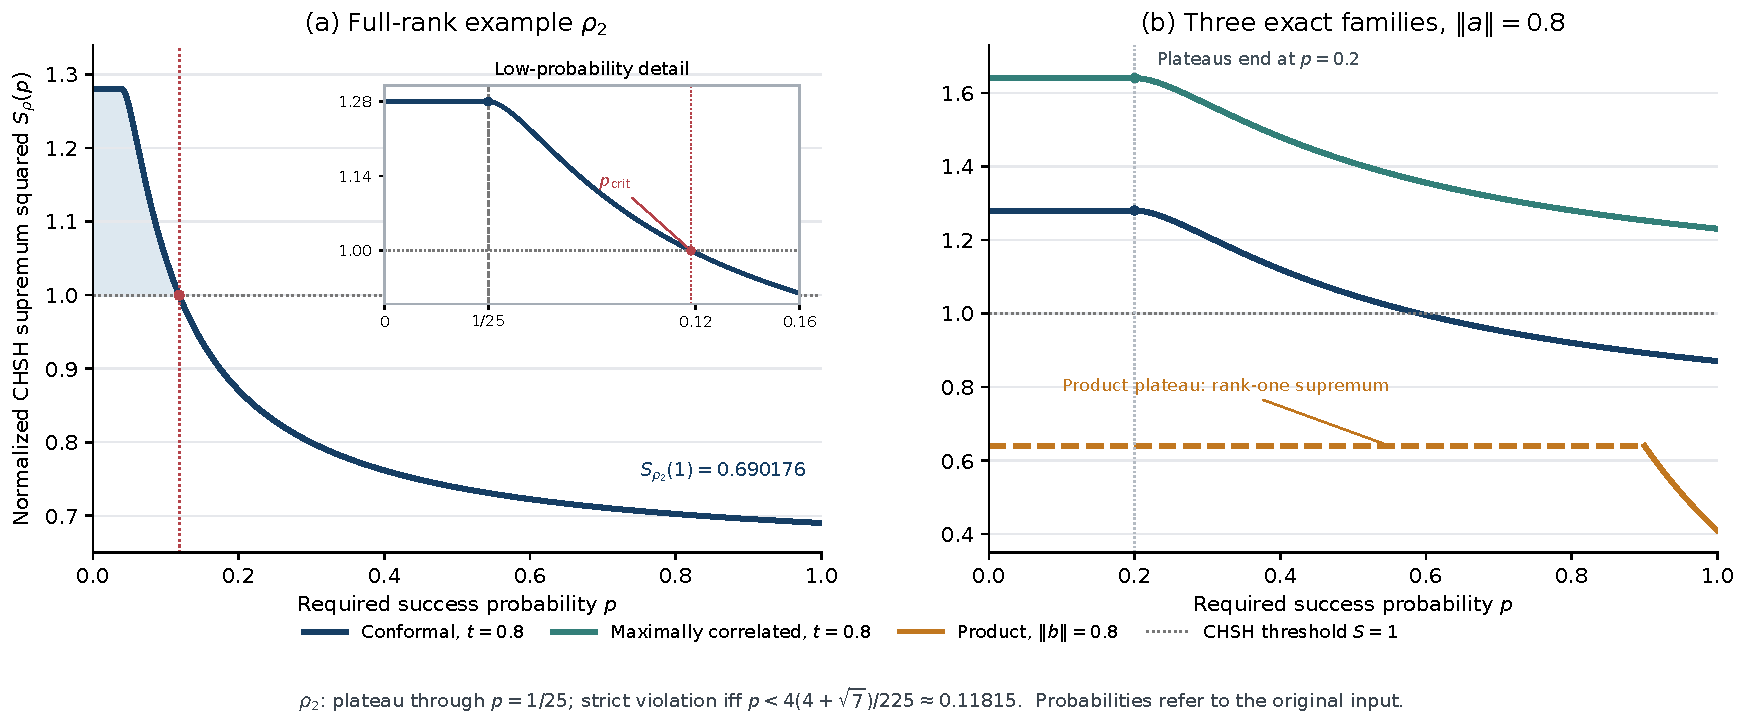
\includegraphics[width=\textwidth]{figures/original_success_frontiers.pdf}
\caption{Exact success frontiers on the original input. The full-rank
$\rho_2$ example violates exactly for required probabilities
$p<4(4+\sqrt7)/225\simeq0.11814669$ and attains its unconstrained score
for $p\le1/25$. The family comparison uses $\norm a=0.8$ and
$t=0.8$ for the conformal and maximally correlated states, and
$\norm b=0.8$ for the product state. The product plateau is a rank-one
supremum; the two entangled-family curves have finite attaining filters.}
\label{fig:r3-frontiers}
\end{figure}
\paragraph{Numerical scope.}
The file \texttt{calculations/original\_input/original\_success.py} evaluates the exact Bob Gram
matrix, projects candidates into the true lens, and performs multistart
optimization over all three effect coordinates. Its general output is
explicitly labeled as a numerical candidate, not a global certificate.
The closed families above and the counterexample are separately checked
using direct complex density matrices and exact symbolic identities.

\section{Convexity, noise scaling, and quantitative stability}
\label{sec:ext-stability}

\begin{proposition}[Convex sublevel sets and a genuine discontinuity]
\label{prop:ext-convexity}
For every $b_0\ge0$, the set $\{\rho:B_A^*(\rho)\le b_0\}$ is convex.
On each affine slice with a fixed Alice marginal, both $B_A^*$ and
$(B_A^*)^2$ are convex functions of $\rho$.
In general $B_A^*$ is neither convex nor continuous at states with
pure filtered-side marginal.
\end{proposition}

\begin{proof}
For a fixed invertible filter, filtering a mixture
$\sum_jq_j\rho_j$ produces the mixture of the individually filtered
states with weights proportional to their success probabilities.
The CHSH norm is convex, because it is the supremum of the appropriate
normalized linear Bell expressions. Its value on the filtered mixture
is therefore at most $\max_j B_A^*(\rho_j)$.
Taking the supremum over filters proves convexity of the sublevel set.

If all $\rho_j$ have the same Alice marginal, each fixed filter has
the same success probability on every component. The weights remain
$q_j$, and taking the supremum proves convexity of $B_A^*$ on the
slice. The square of a nonnegative convex function is convex,
giving the second assertion.

For the last statement, consider
\[
 \rho_p=p|\Phi^+\rangle\langle\Phi^+|
 +(1-p)|0\rangle\langle0|\otimes I/2.
\]
At $p=0$, Alice is pure and Bob maximally mixed, so $B_A^*(\rho_0)=0$.
For $0<p\le1/2$,
$\Delta_B(\rho_p)=p(2p-1)/2\le0$, which gives the upper bound one.
A rank-one Alice filter onto $|1\rangle$ removes the second component
and leaves Bob pure, giving the matching supremum one.
Thus $B_A^*(\rho_p)=1$ throughout $0<p\le1/2$.
It jumps at zero and exceeds the convex interpolation
$pB_A^*(|\Phi^+\rangle)=p\sqrt2$ for, for example, $p=1/4$.
\end{proof}

\begin{proposition}[Exact noise scaling on the unfiltered party]
\label{prop:ext-noise}
Let $\mathcal D_\eta(X)=\eta X+(1-\eta)\tr(X)I/2$ be the
depolarizing channel, with $0\le\eta\le1$. Then
\begin{equation}
 \boxed{
 B_A^*((\mathrm{id}\otimes\mathcal D_\eta)(\rho))
 =\eta B_A^*(\rho).
 }
 \label{eq:ext-noise-scaling}
\end{equation}
For $\eta>0$, the optimal Alice filters are unchanged.
If the original optimum exceeds one, the exact surviving-violation
threshold is $\eta>1/B_A^*(\rho)$.
For a canonical state the same statement applies to admixture of
global white noise.
\end{proposition}

\begin{proof}
Alice filtering commutes with the trace-preserving channel on Bob,
and the filtering success probability is unchanged.
For every normalized filtered state, the channel multiplies its
correlation matrix by $\eta$, and hence its CHSH norm by $\eta$.
The equality follows after taking suprema.
If $\rho_A=I/2$, then
$(\mathrm{id}\otimes\mathcal D_\eta)(\rho)
=\eta\rho+(1-\eta)I/4$, proving the last statement.
For a noncanonical state, global white noise does not generally
obey this scaling law.
\end{proof}

\begin{proposition}[A universal canonical Lipschitz estimate]
\label{prop:ext-lipschitz}
Let $S,S'$ be the squared unilateral optima of two canonical states,
with derived data $(A,s,d)$ and $(A',s',d')$. Then
\begin{equation}
 \boxed{
 |S-S'|\le
 2\norm{A-A'}_{\mathrm{op}}+|s-s'|+2\norm{d-d'}.
 }
 \label{eq:ext-lipschitz}
\end{equation}
This estimate requires no spectral gap and includes all singular
and repeated-eigenvalue cases.
\end{proposition}

\begin{proof}
For a common feasible pair, put $u=-n\times v$ and
$P=I-nn^T-vv^T$. Because $n\cdot v=0$, $\norm n=1$, and
$\norm v\le1$, the matrix $P$ is positive semidefinite and
$\tr P=2-\norm v^2\le2$. The objective is
\[
 f(n,v)=\tr(PA)+s\norm v^2+2u\cdot d.
\]
Since $\norm u=\norm v\le1$, the absolute difference of the
two objectives is bounded by the right-hand side of
\eqref{eq:ext-lipschitz}, uniformly over the common compact domain.
Taking maxima in both orders proves the claim.
\end{proof}

For example, an estimated value $\widehat S$ with certified right-hand
side at most $\varepsilon$ proves activation if
$\widehat S-\varepsilon>1$, and excludes activation if
$\widehat S+\varepsilon\le1$.
The estimate is in canonical coordinates; it does not assert uniform
continuity of whitening as a marginal approaches purity.

\begin{proposition}[Gradients at a simple optimum]
\label{prop:ext-gradient}
Suppose $H_0\succ0$ and the smallest eigenvalue of $M$ is simple.
Choose its normalized eigenvector $n$, put
$v=-K^{-1}Cn$, $u=-n\times v$, and
$P=I-nn^T-vv^T$. Then $S=(B_A^*)^2$ is differentiable in the
canonical data and
\begin{equation}
 \boxed{
 \nabla_D S=2(PD+uc^T),\qquad
 \nabla_c S=2(D^Tu+\norm v^2c).
 }
 \label{eq:ext-gradients}
\end{equation}
\end{proposition}

\begin{proof}
Under the stated hypotheses the optimizing reduced pair is unique up
to the simultaneous sign change $(n,v)\mapsto(-n,-v)$, which leaves
$P$ and $u$ unchanged. The simple-eigenvalue formula is smooth locally.
Equivalently, differentiating the maximized objective while holding
an optimizing pair fixed gives the same derivative.
In
$f=\tr(PDD^T)+\norm c^2\norm v^2+2u^TDc$,
differentiation with respect to $D$ and $c$ gives precisely
\eqref{eq:ext-gradients}.
\end{proof}

\paragraph{Independent checks and scope.}
The accompanying independent script tests these extensions through
complex $4\times4$ density-matrix calculations, separately from the
reference solver. With the recorded seed it checks the Gram identity,
plane-purity identity, determinant covariance, rational ellipsoid data,
and scalar probability formula on $1{,}000$ states of ranks one through
four. It tests $417$ purity-positive shortcut instances, $600$ physical
axial states, and $102$ success-frontier comparisons against direct
multistart filtering. The largest shortcut-attainment discrepancy is
$2.7\times10^{-15}$ and the largest frontier discrepancy is
$8.2\times10^{-10}$.
Further checks cover $1{,}000$ independent random rank-two states,
$129$ rational-cubic value evaluations, and $11$ points of the exact
tilted frontier. The rank-two ceiling discrepancy is below
$1.8\times10^{-15}$; the explicit tilted filters agree with direct
optimization within $2.9\times10^{-15}$.
These numerical checks support the mathematical
proofs; they do not establish them or extend the Lean coverage.
The exact formalization boundary is stated separately in
Appendix~\ref{sec:verification}.


\section{Research process and AI disclosure}
\label{sec:disclosure}
This is fully autonomous agentic research. The results, their proofs, the
Lean development, the exact and numerical checkers and a draft report were
produced by autonomous AI research agents in an earlier session; its records
describe internal reviews carried out within the same automated workflow
and do not name the system used.

Opus~5.5 by Anthropic used with Claude Code assessed the work for this
release. It confirmed that the problem solved is Eq.~(9) of~\cite{ducuara},
read the proofs of the compact reduction, the Gram identity, the
least-eigenvalue theorem and the violation criterion, compared the Lean
definitions and endpoint statements with the mathematics, ran the fresh
Lean build and the whole-project axiom audit recorded in
\texttt{verification/}, reran every checker from a copy, wrote the
independent check \texttt{calculations/release\_check.py}, read the Omega
Institute's dossier on Conjecture~1, and edited and reorganized this
manuscript from the draft report, adding the introduction, the main-results
summary and the priority notes. The mathematical statements of the draft
were not changed. The remaining proofs were carried over and read, but not
all were rederived line by line.

Dev D. Goyal is responsible for publication. The work has not been
externally peer reviewed; AI checks are not human peer review, no expert
validation is claimed, and the literature comparison is bounded and does
not establish priority. Appendix~\ref{sec:verification} states the formal
scope and its limits.

\appendix
\section{Proof of the finite-candidate theorem}
\label{sec:proof-general}

Section~\ref{sec:compact} reduced the problem to the maximum~\eqref{eq:compactreduction} and showed that the boundary maximum is $E$ and that interior maxima satisfy the pencil equations~\eqref{eq:stationary}. It remains to analyse the pencil.

\subsection{Why the pencil is a cubic with real roots}

Both $\HH$ and $\BB$ annihilate $\mathcal L_0$ and preserve its orthogonal complement. Their restrictions have no common kernel. If
$(\widehat H-i\widehat B)z=0$, its Hermitian inner product with $z$ has imaginary part $-z^*\widehat Bz=0$. Positive semidefiniteness of $\widehat B$ implies $\widehat Bz=0$ and then $\widehat Hz=0$, a contradiction. Thus $p(i)\ne0$, so $p$ is nonzero. Its degree is at most $\rank\widehat B\le3$.

If $(\widehat H-\lambda\widehat B)z=0$ for a nonzero complex $z$, then $z^*\widehat Bz>0$ by the same common-kernel argument. Hence
\begin{equation}
 \lambda=\frac{z^*\widehat Hz}{z^*\widehat Bz}\in\R.
\end{equation}
Moreover, projecting an eigenspace representative onto its first three coordinates is injective; a representative with $n=0$ would lie in the removed common kernel. Thus every reduced eigenspace has dimension at most three.

\subsection{The feasibility test and the exceptional level}
\label{sec:phase}

For $\lambda\ne s$,~\eqref{eq:stationaryvalue} already forces $n^Tv=0$. A nonzero solution can be normalized to $\norm n=1$, $\norm v\le1$ exactly when some solution has
\begin{equation}
 \norm n^2-\norm v^2\ge0.
\end{equation}
Adding a common-kernel vector changes only the component of $v$ in $\ker K\cap\ker C$. Removing that component maximizes the displayed difference. The existence test is therefore exactly $\chi_\lambda\ge0$, and its strict version gives $\norm v<1$.

At $\lambda=s$, the equations are the real and imaginary parts of
\begin{equation}
 (K+iC)(n+iv)=0.
 \label{eq:complexkernel}
\end{equation}
They are invariant under multiplication of $n+iv$ by a complex phase. Choose that phase so that the real and imaginary parts are orthogonal and the real part has at least the imaginary part's norm. This is just diagonalization of the real $2\times2$ Gram matrix of $n,v$. Then normalize the real part to norm one. The resulting pair belongs to $\mathcal D$ and has the required value. If $\chi_s>0$, the phase can give strict inequality of norms. Conversely, an interior representative has a positive $\JJ$-quadratic form, so it implies $\chi_s>0$ after removing the common-kernel component.

An equivalent exact strict test is useful in implementations: for any complex basis matrix $Q_c$ of $\ker(K+iC)$, the exceptional level has an interior representative if and only if
\begin{equation}
 Q_c^TQ_c\ne0.
 \label{eq:nonisotropic}
\end{equation}
Indeed $z^Tz\ne0$ means that a phase can make $z^Tz$ positive real, giving orthogonal real and imaginary parts with unequal norms. If all these bilinear squares vanish, every phase-normalized representative is on the boundary. This handles repeated eigenvalues without choosing an arbitrary real eigenvector.

Every admissible spectral level therefore has a feasible representative, while every interior maximum is among those levels. Together with the boundary maximum, this proves Theorem~\ref{thm:main}.

\subsection{Justification of the singular compression}
From $Kv=-Cn$ we obtain $n\perp C\ker K$, so $n\in\ran P$. The general solution is
$v=-K^\dagger Cn+Nw$. Substitution into the first stationary equation yields
\begin{equation}
 (M_0-\lambda I)n=CNw.
\end{equation}
Projecting to $(C\ker K)^\perp$ gives exactly the eigenproblem for $M_L$. The residual lies in $\ran(CN)$, and the minimum-norm solution for $w$ gives~\eqref{eq:V}. All remaining freedom is a vector in $\ker K\cap\ker C$, which only increases $\norm v$ from its minimum. For $\lambda\ne s$, orthogonality to $n$ is automatic for every such solution. This proves the stated singular-value test and demonstrates that no regularization limit is hidden in the formula.

\section{Verification and formal scope}
\label{sec:verification}

\subsection{What the Lean development proves}

The Lean project in \path{lean/} pins Lean~4.19.0 and Mathlib revision
\path{c44e0c8ee63ca166450922a373c7409c5d26b00b}. Its $32$ proof modules
use the following definitions. A state is a matrix
$\rho\in\C^{4\times4}$, indexed by pairs of qubit indices, with the
hypotheses that $\rho$ is positive semidefinite (Mathlib's
\texttt{PosSemidef}) and has trace one. An Alice filter is any
$F\in\C^{2\times2}$ with $\det F\ne0$; the filtered state is
$(F\otimes I)\rho(F\otimes I)^\dagger$ divided by the real part of its
trace, and the development proves that this trace is positive and that the
result is again a density matrix. Bob filters act on the second factor.
A measurement observable is a $2\times2$ complex matrix $O$ with
$O^\dagger=O$, $O^2=I$ and $\tr O=0$; this is proved equivalent to
$O=\hat u\cdot\sigma$ for a unit vector $\hat u$. The value attached to a
filter and four observables is the square of
$\Re\tr(\rho'\mathcal B)/2$, where $\mathcal B$ is the usual Bell operator,
so that the local bound is $1$; the measure is the supremum (least upper
bound) of these values. As in~\cite{ducuara}, filters are not required to
be contractions: a scalar multiple of a filter gives the same normalized
state.

\begin{table}[h]
\centering\small
\begin{tabular}{@{}>{\raggedright\arraybackslash}p{0.43\textwidth}>{\raggedright\arraybackslash}p{0.51\textwidth}@{}}
\toprule
Statement & Lean declaration (namespace \path{UnilateralCHSH.Quantum}) \\
\midrule
Result A: both one-sided suprema, every state, arbitrary observables
 & \path{all_states_operator_both_isLUB} \\
Pure filtered marginal: value $\norm b^2$, attained
 & \path{pure_marginal_gl_isGreatest} \\
Result B: least-eigenvalue formula for $\alpha>1$ with an attaining filter
 & \path{all_states_alice_schur_formula} \\
Result C: violation criterion (Alice, Bob)
 & \path{all_states_alice_operator_activation_iff},
   \path{all_states_bob_operator_activation_iff} \\
Hidden one-sided activation
 & \path{all_states_alice_operator_hidden_activation_iff} and the Bob version \\
Invertible attainment of a violating supremum
 & \path{all_states_alice_operator_violation_attained} and the Bob version \\
Result D: at most four candidates (boundary value and spectral levels)
 & \path{original_finite_candidates} \\
Whitening in explicit coordinates, orbit equality
 & \path{original_filter_orbit_explicit} \\
Bob's measure from Alice's by an actual qubit swap
 & \path{bobGLValues_eq_alice_swap} \\
\bottomrule
\end{tabular}
\end{table}

In these statements the value of the supremum is the function
\texttt{aliceMaximum}: for a mixed Alice marginal it is the maximum of the
reduced objective~\eqref{eq:f} over the compact domain~\eqref{eq:domain},
evaluated at the whitened coordinates, and for a pure marginal it is
$\norm b^2$. The least-eigenvalue statement asserts $\det K\ne0$ and
produces $r>0$ and a unit vector $n$ with $(K+CK^{-1}C)n=rn$, $r\norm x^2\le
x^{\mathsf T}(K+CK^{-1}C)x$ for every $x$, value $\alpha-r$, and an
invertible filter attaining it; with $M-sI=K+CK^{-1}C$ this is
Result~B. The violation criterion is stated as $\norm a<1$, $\alpha>1$ and
the existence of a unit vector $n$ with
$n^{\mathsf T}(K+CK^{-1}C)n<\alpha-1$, which is
$\lambda_{\min}(M)<\tr A-1$. Along the way the development proves the
compact attainment and Lagrange conditions derived from actual
maximality, the finite spectral candidates including all singular cases,
the reduction of every filter and measurement plane, the Gram identity and
purity guard, the Horodecki plane formula with explicit attaining
measurements, local-unitary invariance, polar factorization of every
invertible filter, the Fano representation, whitening and its inverse,
continuity and radial approximation of the supremum, and product
factorization at a pure marginal.

\paragraph{Audit.} The audit module \texttt{UnilateralAxiomAudit}
enumerates every declaration whose defining module is one of the $32$
proof modules and collects its axioms with Lean's \texttt{collectAxioms}.
In the fresh build recorded in \path{verification/} it covers $1{,}060$
declarations. The $869$ declarations other than code-generation
auxiliaries are not axioms and depend only on \texttt{propext},
\texttt{Classical.choice} and \texttt{Quot.sound}; the other $191$ are
auxiliary declarations that the Lean~4.19 code generator stores for
executable definitions, $12$ of which refer to its placeholder
\texttt{lcProof}, which the audit permits for such auxiliaries only. All
$730$ named source declarations were audited, and the sources contain no
\texttt{sorry}, \texttt{admit}, \path{native_decide},
\texttt{ofReduceBool}, \path{implemented_by}, \texttt{extern},
\texttt{unsafe} or \texttt{axiom}.

\subsection{What is conventional}

The following have conventional proofs in this paper, with the exact and
numerical checks listed below, but are not formalized: the explicit
evaluation of the boundary radius $E$ by the secular equation and its hard
case (Section~\ref{sec:boundary}), the explicit cubic, the admissibility
tests and the singular compression of Section~\ref{sec:formula} (the formal
finite-candidate theorem uses an attained maximum over the sphere and the
eligible spectral levels); the polynomial and rational-ellipsoid
activation tests and the rational cubic (Section~\ref{sec:ext-polynomial});
the three regimes at $B_A^*=1$ and the product-kernel criterion; the
rank-two formula, which uses the Ruskai--Szarek--Werner
classification~\cite{ruskai2002}; the characterization of $B_A^*=\sqrt2$;
the axial family and the quasi-distillable family; all success-probability
results of Sections~\ref{sec:ext-probability} and~\ref{sec:r3-success};
and the convexity, scaling and stability results of
Section~\ref{sec:ext-stability}. The extension of Result~B to the
hypothesis $K+iC\succ0$ is also conventional.

\subsection{Exact and numerical checks}

The directory \path{calculations/} contains the checkers and their
recorded outputs; \path{scripts/run_checks.py} replays all of them in a
temporary copy with \texttt{python3 -I} and compares each output with the
record. They are falsification attempts and exact checks of particular
instances; no theorem rests on them.

\begin{itemize}[leftmargin=1.5em]
\item \path{exact_examples.py}: exact SymPy verification of positivity,
Bloch data, candidate eigenvalues, filters, success probabilities and output
correlations for the examples of Section~\ref{sec:attainment} and the
following sections, and of the symbolic pencil determinant identity.
\item \path{audit_spectral_cases.py}: $655$ canonical data sets, including
$\rank K\in\{0,1,2\}$, common kernels, repeated eigenvalues and vanishing
centres, with an independent spectral reconstruction and $252{,}500$ sampled
filters; reconstructed witnesses match to about $10^{-13}$ and no sampled
filter exceeds the formula.
\item \path{independent_audit/check_spectral.py}: $275$ comparisons of the
formula with multistart direct filtering of complex density matrices
(canonical states of ranks one to four, original states for both parties,
singular cases, exact examples); direct optimization never exceeds the
formula by more than roundoff, with a largest gap of about
$4.4\times10^{-8}$ consistent with approaching a boundary supremum.
\item \path{extensions/independent_checks.py}: $1{,}000$ states of ranks
one to four for the Gram, plane-purity, covariance and ellipsoid identities;
$417$ guard-region instances; $600$ axial states; $102$ success-frontier
comparisons with direct filtering; the counterexample showing that $K\succ0$
alone does not suffice.
\item \path{extensions/additional_exact_checks.py},
\path{rank2_checks.py}, \path{nonunique_optimizer_example.py},
\path{bilateral_family_certificate.py}: the rational cubic on sampled
states, $1{,}000$ rank-two states, an exact circle of optimal filters, and
an exact certificate for the bilateral filter of the quasi-distillable
family at $p=3/5$.
\item \path{original_input/}: $256$ original states with $512$ arbitrary
complex filter comparisons for the whitening formulas, and the
original-input success lens, Gram matrix and closed frontiers.
\item \path{check_extensions.py}: tests of the public solver functions,
including exact activation signs and exact cubic roots.
\item \path{check_filter_reduction.py}: $2{,}000$ instances of the real
filter reduction used in the formal proof.
\item \path{release_check.py}, written for this release without importing
the other files: exact values for $\rho_1$, $\rho_2$ and the
quasi-distillable family on the grid $p=k/12$, the explicit optimal filter
of $\rho_1$ applied to the density matrix, and $160$ random states of ranks
one to four with $\alpha>1$, for which the least-eigenvalue value agrees
with the reconstructed invertible filter and with multistart direct
maximization to about $10^{-13}$.
\end{itemize}

\paragraph{Numerical rank caution.}
The reference solver uses floating-point eigensolvers and tolerances and is
not an exact certificate near degeneracies. There is a genuine
discontinuity at a pure filtered-side marginal: for
$\sqrt{1-\varepsilon}|00\rangle+\sqrt\varepsilon|11\rangle$, every
$\varepsilon>0$ has $B_A^*=\sqrt2$, whereas $\varepsilon=0$ has value $1$.
Treating a small positive marginal eigenvalue as zero can therefore produce
an order-one error; the solver refuses unsafe near-singular marginal
decisions instead of returning a product-state answer.


\begin{thebibliography}{99}
\bibitem{ducuara} A.~F.~Ducuara, C.~E.~Susa and P.~Skrzypczyk,
\emph{Locally inaccessible hidden quantum correlations}, Phys.\ Rev.\ A
\textbf{110}, 022435 (2024),
\href{https://arxiv.org/abs/2406.03945}{arXiv:2406.03945}.
\bibitem{horodecki1995} R.~Horodecki, P.~Horodecki and M.~Horodecki,
\emph{Violating Bell inequality by mixed spin-$\frac12$ states: necessary
and sufficient condition}, Phys.\ Lett.\ A \textbf{200}, 340--344 (1995),
\href{https://doi.org/10.1016/0375-9601(95)00214-N}{doi:10.1016/0375-9601(95)00214-N}.
\bibitem{verstraete} F.~Verstraete, J.~Dehaene and B.~De~Moor,
\emph{Local filtering operations on two qubits}, Phys.\ Rev.\ A \textbf{64},
010101(R) (2001),
\href{https://arxiv.org/abs/quant-ph/0011111}{arXiv:quant-ph/0011111}.
\bibitem{verstraetewolf} F.~Verstraete and M.~M.~Wolf,
\emph{Entanglement versus Bell violations and their behavior under local
filtering operations}, Phys.\ Rev.\ Lett.\ \textbf{89}, 170401 (2002),
\href{https://arxiv.org/abs/quant-ph/0112012}{arXiv:quant-ph/0112012}.
\bibitem{klm} A.~Kent, N.~Linden and S.~Massar,
\emph{Optimal entanglement enhancement for mixed states}, Phys.\ Rev.\
Lett.\ \textbf{83}, 2656--2659 (1999),
\href{https://arxiv.org/abs/quant-ph/9902022}{arXiv:quant-ph/9902022}.
\bibitem{palghosh} R.~Pal and S.~Ghosh,
\emph{A closed-form necessary and sufficient condition for any two-qubit
state to show hidden nonlocality w.r.t.\ the Bell--CHSH inequality},
\href{https://arxiv.org/abs/1410.7574}{arXiv:1410.7574} (2014).
\bibitem{li2017} M.~Li et al.,
\emph{Maximal violation of Bell inequalities under local filtering},
Sci.\ Rep.\ \textbf{7}, 46505 (2017),
\href{https://doi.org/10.1038/srep46505}{doi:10.1038/srep46505},
\href{https://arxiv.org/abs/1704.08142}{arXiv:1704.08142}.
\bibitem{zhang} Y.~Zhang, R.~Araiza Bravo, V.~O.~Lorenz and E.~Chitambar,
\emph{Channel activation of CHSH nonlocality}, New J.\ Phys.\ \textbf{22},
043003 (2020),
\href{https://doi.org/10.1088/1367-2630/ab7bef}{doi:10.1088/1367-2630/ab7bef},
\href{https://arxiv.org/abs/1911.06349}{arXiv:1911.06349}.
\bibitem{kumari} S.~Kumari et al.,
\emph{Interplay of nonlocality and incompatibility breaking qubit channels},
Phys.\ Rev.\ A \textbf{107}, 022201 (2023),
\href{https://arxiv.org/abs/2210.02744}{arXiv:2210.02744}.
\bibitem{horodecki1996} R.~Horodecki, P.~Horodecki and M.~Horodecki,
\emph{Quantum $\alpha$-entropy inequalities: independent condition for
local realism?}, Phys.\ Lett.\ A \textbf{210}, 377--381 (1996),
\href{https://doi.org/10.1016/0375-9601(95)00930-2}{doi:10.1016/0375-9601(95)00930-2}.
\bibitem{ruskai2002} M.~B.~Ruskai, S.~Szarek and E.~Werner,
\emph{An analysis of completely-positive trace-preserving maps on $M_2$},
Linear Algebra Appl.\ \textbf{347}, 159--187 (2002),
\href{https://arxiv.org/abs/quant-ph/0101003}{arXiv:quant-ph/0101003}.
\bibitem{more} J.~J.~Mor\'e and D.~C.~Sorensen,
\emph{Computing a trust region step}, SIAM J.\ Sci.\ Stat.\ Comput.\
\textbf{4}, 553--572 (1983),
\href{https://doi.org/10.1137/0904038}{doi:10.1137/0904038}.
\bibitem{holscherer2005} C.~W.~J.~Hol and C.~W.~Scherer,
\emph{Sum of squares relaxations for robust polynomial semi-definite
programs}, Proc.\ 16th IFAC World Congress (2005), Theorem~2.
\bibitem{milne} A.~Milne, D.~Jennings, S.~Jevtic and T.~Rudolph,
\emph{Quantum correlations of two-qubit states with one maximally mixed
marginal}, Phys.\ Rev.\ A \textbf{90}, 024302 (2014),
\href{https://arxiv.org/abs/1404.3951}{arXiv:1404.3951}.
\bibitem{jevtic} S.~Jevtic, M.~Pusey, D.~Jennings and T.~Rudolph,
\emph{Quantum steering ellipsoids}, Phys.\ Rev.\ Lett.\ \textbf{113},
020402 (2014), \href{https://arxiv.org/abs/1303.4724}{arXiv:1303.4724}.
\bibitem{dossier} The Omega Institute, \emph{CHSH nonlocality is tightly
bounded by the steering-ellipsoid centre}, problem dossier and Lean source,
repository \texttt{the-omega-institute/trureturing}, issue \#16558; dossier
committed 14 October 2026 (commit \texttt{af41108}),
\url{https://github.com/the-omega-institute/trureturing/blob/af41108edc85c119837189f120c6d2d9aa3f5a25/Problems/milne-jennings-jevtic-rudolph-2014-chsh-centre-bound.md}.
\end{thebibliography}
\end{document}
